\label{cap:Apresetacao}

Nesse capítulo iremos apresentar os dados coletados em laboratório junto com a análise que obtivemos do comportamento do servidor Memcached no ataque. De forma geral os testes seguiram a metodologia descrita em Gondim et al. \cite{Gondim2016} na avaliação de ataques DDoS.

\section{Coleta de dados}
\label{sec:Coleta}
Todas as capturas foram feitas em um ambiente controlado utilizando o analisador de protocolos de rede TShark para fazer a captura e análise do tráfego de rede. A configuração das máquinas é apresentada no tabela \ref{tab:ConfMaq}. O roteador utilizado foi o ASUS RT-AC1900 de 1Gbit/s e a versão do Memcached utilizada foi a 1.5.10 .

Cada nível do ataque tem uma duração de 5 segundos. Para obter o valores de bytes e pacotes de um nível específico foi feita a média aritmética de 5 em 5 segundos da estatística retornado pelo TShark de cada captura.
 
\begin{table}[H]
\label{tab:ConfMaq}
\caption{Configuração das máquinas utilizadas}
\begin{tabular}{|l|l|l|l|l|}
\hline
         & Processador         & Ram & Placa de rede           & SO               \\ \hline
Sputnik  & AMD Ryzen 7 1700    & 16G & 1Gbit/s & Manjaro Linux 18 \\ \hline
Spitfire & Intel Core i5-6200U & 12G & 1Gbit/s & Manjaro Linux 18 \\ \hline
Orion    & Inter Core i7-6700  & 16G & 1Gbit/s & Manjaro Linux 18 \\ \hline
\end{tabular}
\end{table}

Para termos uma melhor análise do comportamento do Memcached no ataque e para minimizar o residual que a diferença de hardware pode deixar na análise optamos por fazer o rodízio das máquinas entre atacante, amplificador e vítima, resultando em 6 possíveis configurações.

Como a maioria dos servidores Memcached que estão expostos na internet estão com a configuração padrão optamos por fazer as mínimas alterações possíveis no amplificador para o teste. A única alteração feita foi a abertura da porta 11211 no protocolo UDP, já que na última versão do Memcached essa porta não vem mais aberta por padrão.

Para cada configuração de ataque iremos apresentar os dados coletados para os dois ataques possíveis no Memcached, o STATS e o GET/SET. Para cada ataque são apresentados dois gráficos, um para os bytes e outro para os pacotes que cada máquina enviou e recebeu e outro gráfico com amplificação para cada nível de ataque. A seguir são apresentas essa tabelas para cada configuração. 

\subsection*{Configuração 1}

Essa configuração se caracteriza por ter o refletor e vítima mais fortes e a atacante mais fraco. 

No método GetSet tivemos um máximo de 63 bytes/pacotes chegando no amplificador no nível 4 e um máximo de 1440.83 bytes/pacotes saindo do amplificador no nível 1 como apresentado na tabela \ref{tab:bytespacsGetSet1}, apesar do atacante saturar apenas no nível 7 como mostra os gráficos \ref{graf:GetSetBytes1} e \ref{graf:GetSetFrames1}.

Já para o método Stats tivemos um máximo de 60.02 bytes/pacotes chegando no amplificador no nível 4 e um máximo de 1003.04 bytes/pacotes saindo do amplificador também no nível 4 como apresentado na tabela \ref{tab:bytespacsStats1}, apesar do atacante saturar apenas no nível 7 como mostra os gráficos \ref{graf:StatsBytes1} e \ref{graf:StatsFrames1}.

\begin{table}[H]
\centering
\caption{Configuração 1}
\begin{tabular}{|l|l|}
\hline
Atacante     & Sputnik  \\ \hline
Refletor     & Spitfire \\ \hline
Vítima       & Orion    \\ \hline
\end{tabular}
\end{table}

\subsubsection{GetSet}

\begin{figure}[H]
     \centering
     \label{graf:GetSetBytes1}
     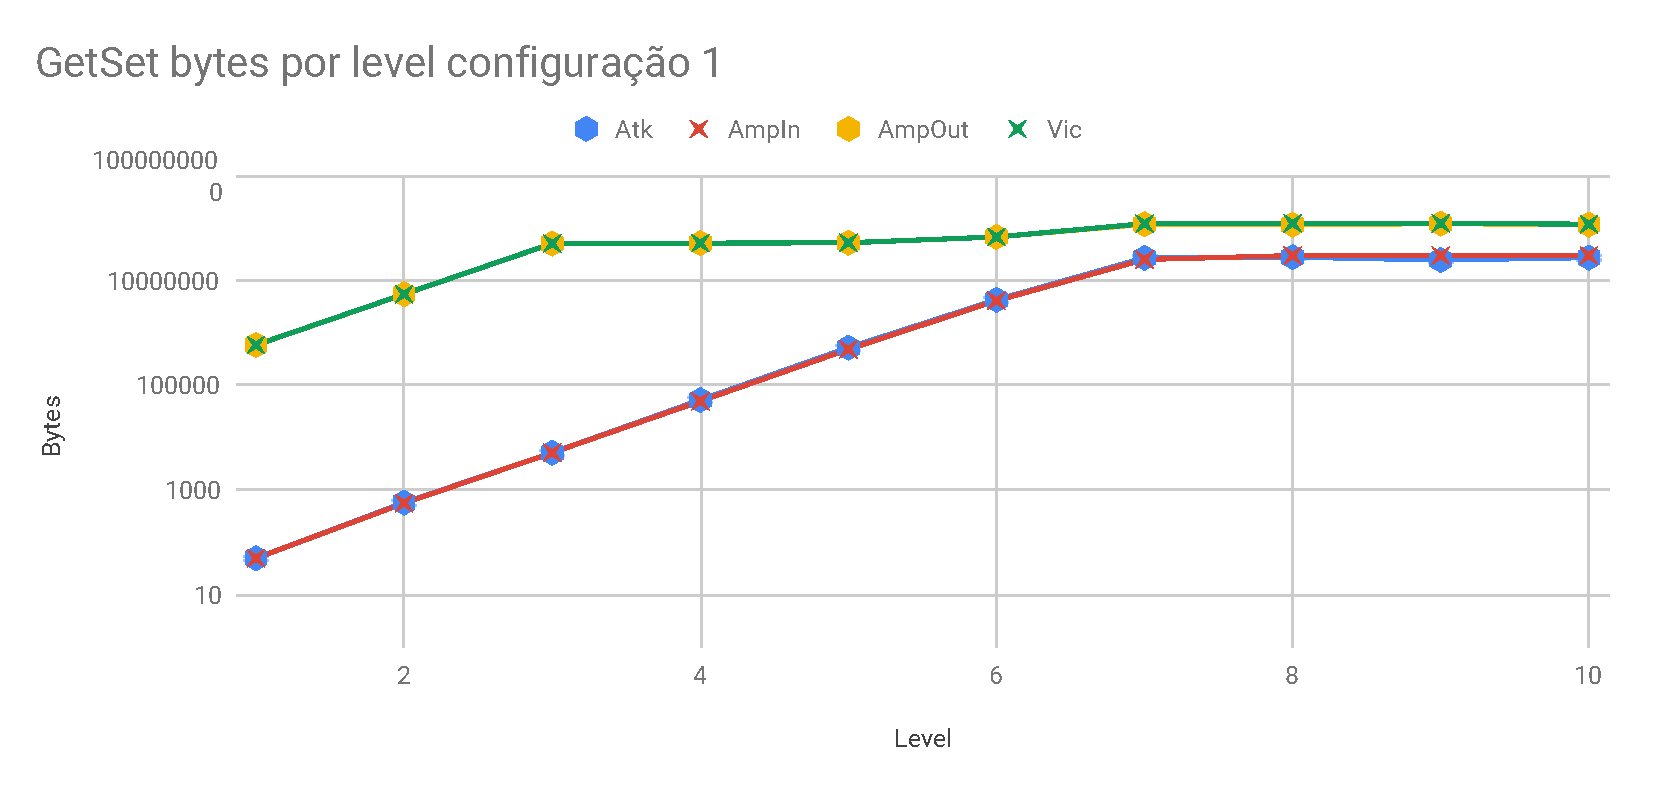
\includegraphics[scale=0.6]{img/capturas/GetSetBLC1.pdf}\
     \caption{GetSet bytes por level configuração 1}
\end{figure}

\begin{figure}[H]
     \centering
     \label{graf:GetSetFrames1}
     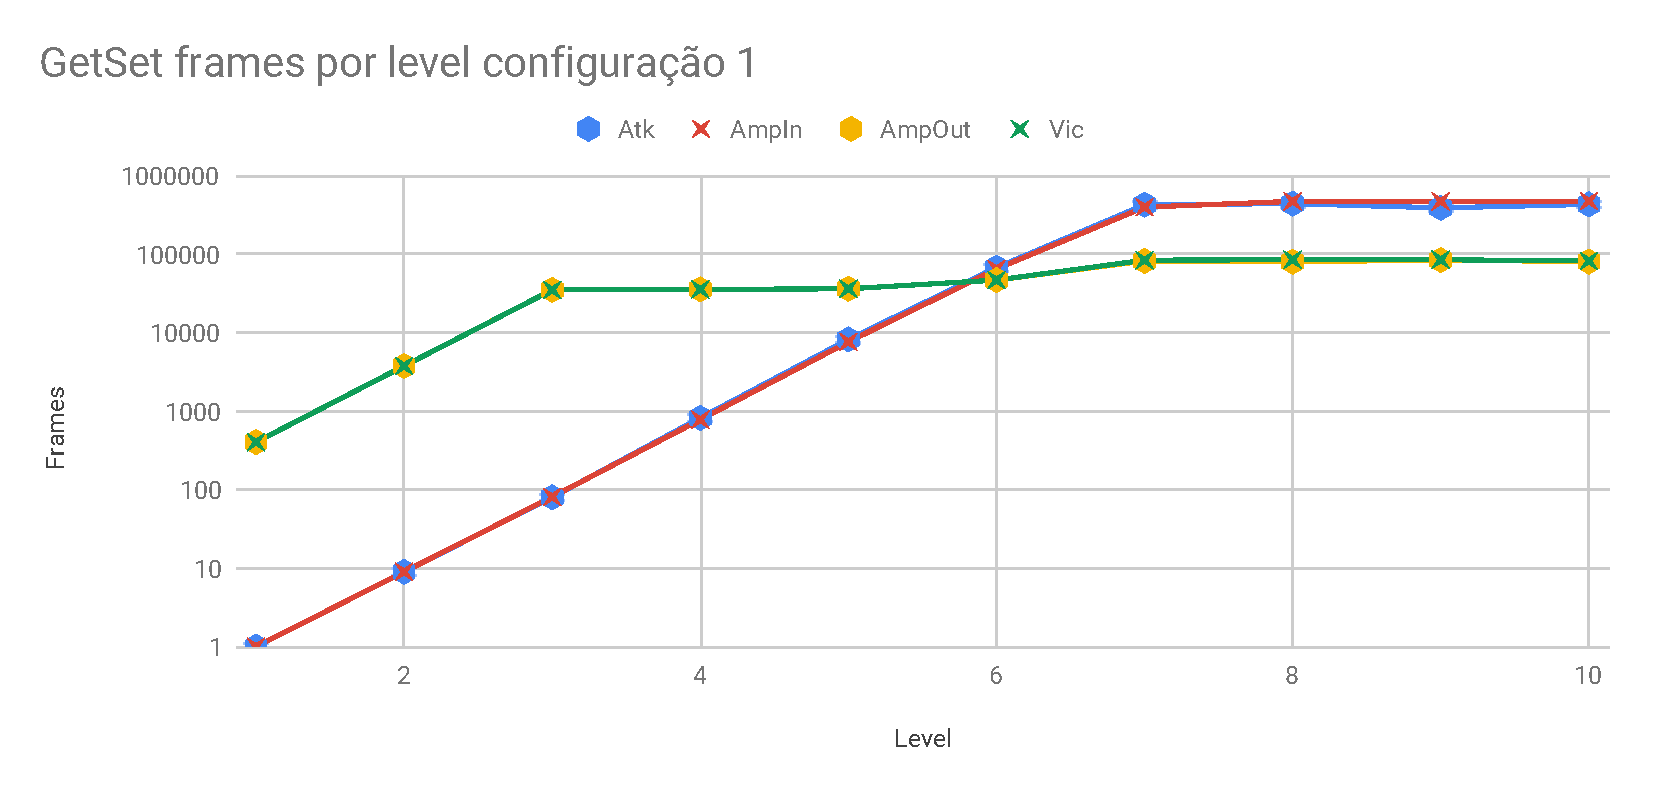
\includegraphics[scale=0.6]{img/capturas/GetSetFLC1.pdf}\
     \caption{GetSet frames por level configuração 1}
\end{figure}

\begin{table}[H]
\centering
\label{tab:bytespacsGetSet1}
\caption{Razão de bytes por pacotes para cada nível no método GetSet configuração 1}
\begin{tabular}{|c|c|c|}
\hline
Nível & Input & Output  \\ \hline
1     & 49.0  & 1440.83 \\ \hline
2     & 61.44 & 1441.01 \\ \hline
3     & 62.83 & 1440.8  \\ \hline
4     & 63.0  & 1440.82 \\ \hline
5     & 63.0  & 1440.78 \\ \hline
6     & 63.0  & 1440.78 \\ \hline
7     & 63.0  & 1440.79 \\ \hline
8     & 63.0  & 1440.79 \\ \hline
9     & 63.0  & 1440.79 \\ \hline
10    & 63.0  & 1440.81 \\ \hline
\end{tabular}
\end{table}

\subsubsection{Stats}

\begin{figure}[H]
     \centering
     \label{graf:StatsBytes1}
     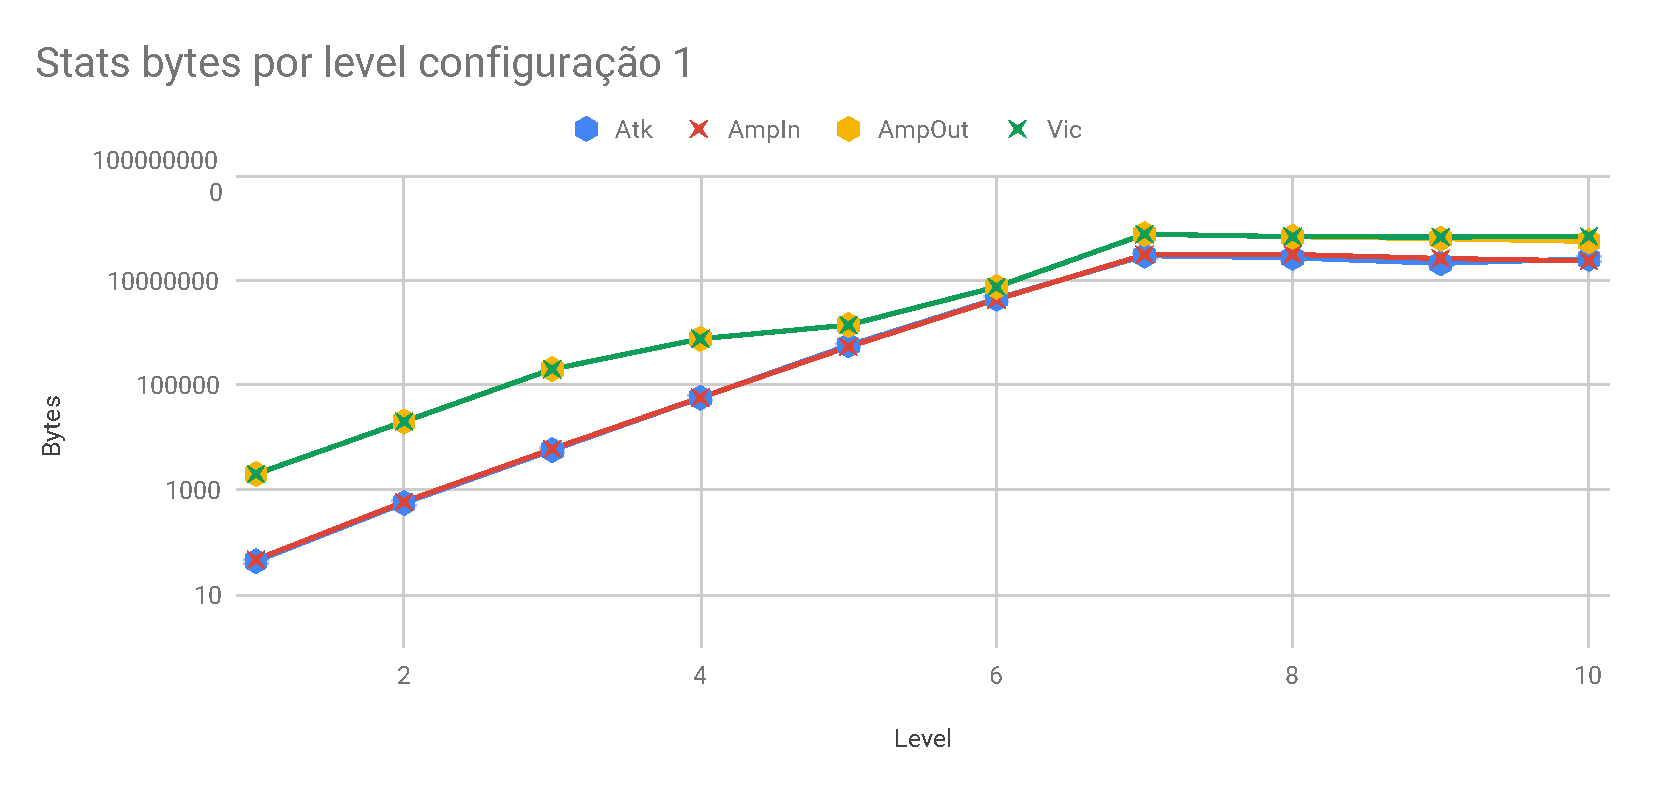
\includegraphics[scale=0.6]{img/capturas/StatsBLC1.pdf}\
     \caption{Stats bytes por level configuração 1}
\end{figure}

\begin{figure}[H]
     \centering
     \label{graf:StatsFrames1}
     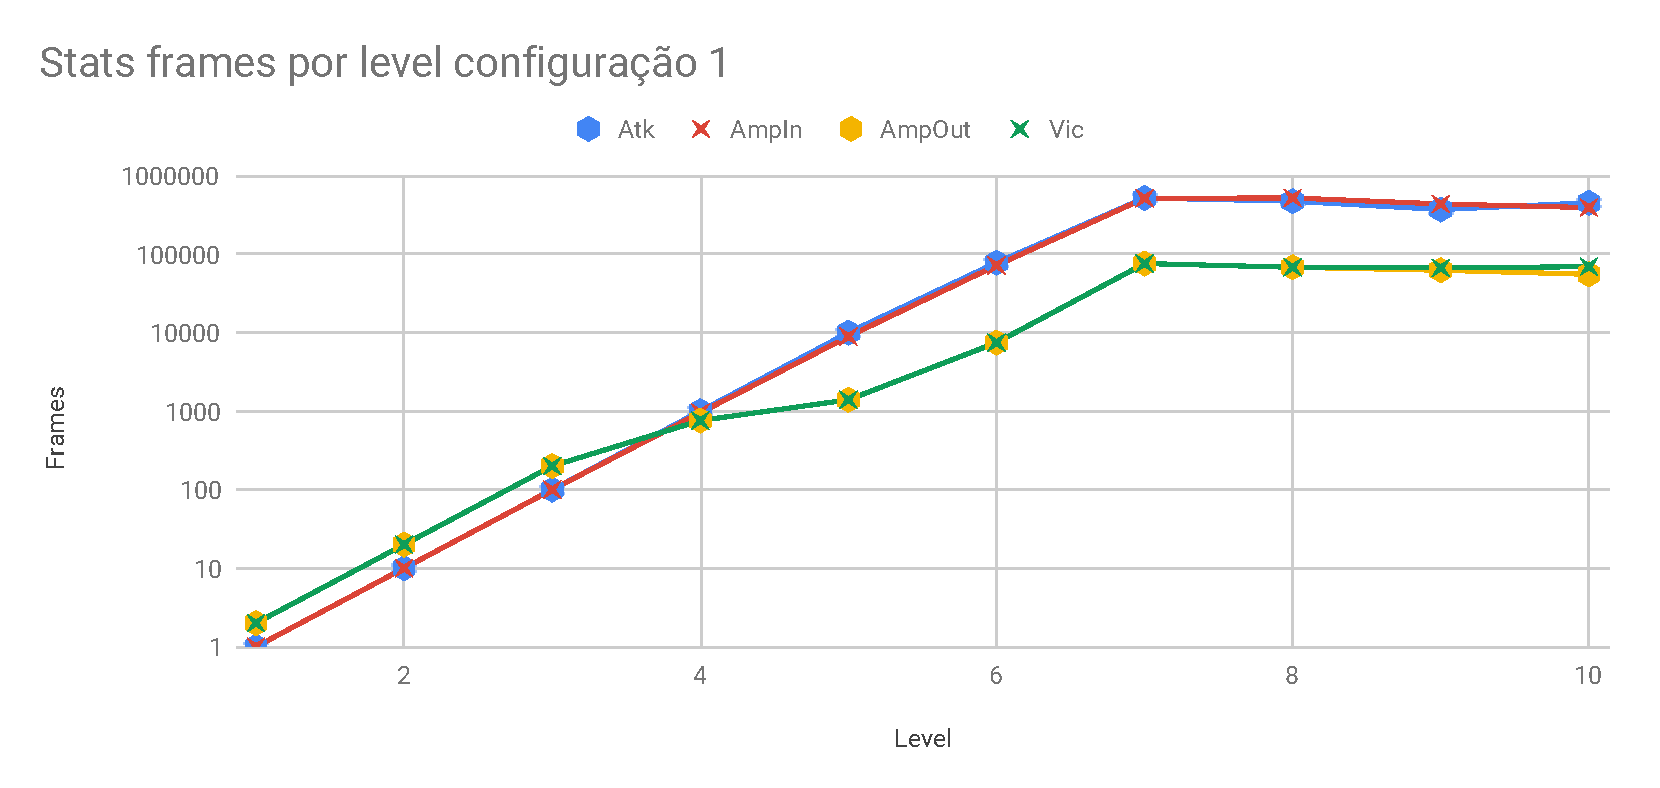
\includegraphics[scale=0.6]{img/capturas/StatsFLC1.pdf}\
     \caption{Stats frames por level configuração 1}
\end{figure}

\begin{table}[H]
\centering
\label{tab:bytespacsStats1}
\caption{Razão de bytes por pacotes para cada nível no método Stats configuração 1}
\begin{tabular}{|c|c|c|}
\hline
Nível & Input & Output  \\ \hline
1     & 46.0  & 995.0   \\ \hline
2     & 58.6  & 1001.3  \\ \hline
3     & 59.86 & 1001.93 \\ \hline
4     & 60.02 & 1003.04 \\ \hline
5     & 60.0  & 1002.13 \\ \hline
6     & 60.0  & 1002.08 \\ \hline
7     & 60.0  & 1002.01 \\ \hline
8     & 60.0  & 1002.01 \\ \hline
9     & 60.0  & 1002.5  \\ \hline
10    & 60.0  & 1002.5  \\ \hline
\end{tabular}
\end{table}

\subsection*{Configuração 2}

Essa configuração se caracteriza por ter o refletor e atacante mais fortes e a vítima mais
fraca.

No método GetSet tivemos um máximo de 63 bytes/pacotes chegando no amplificador no nível 5 e um máximo de 1440.8 bytes/pacotes saindo do amplificador no nível 7 como apresentado na tabela \ref{tab:bytespacsGetSet2}, apesar do atacante saturar apenas no nível 8 como mostra os gráficos \ref{graf:GetSetBytes2} e \ref{graf:GetSetFrames2}.

Já para o método Stats tivemos um máximo de 60.04 bytes/pacotes chegando no amplificador no nível 4 e um máximo de 1020.93 bytes/pacotes saindo do amplificador também no nível 4 como apresentado na tabela \ref{tab:bytespacsStats2}, apesar do atacante saturar apenas no nível 7 como mostra os gráficos \ref{graf:StatsBytes2} e \ref{graf:StatsFrames2}.

\begin{table}[H]
\centering
\caption{Configuração 2}
\begin{tabular}{|l|l|}
\hline
Atacante     & Spitfire  \\ \hline
Refletor     & Orion     \\ \hline
Vítima       & Sputnik   \\ \hline
\end{tabular}
\end{table}

\subsubsection{GetSet}

\begin{figure}[H]
     \centering
     \label{graf:GetSetBytes2}
     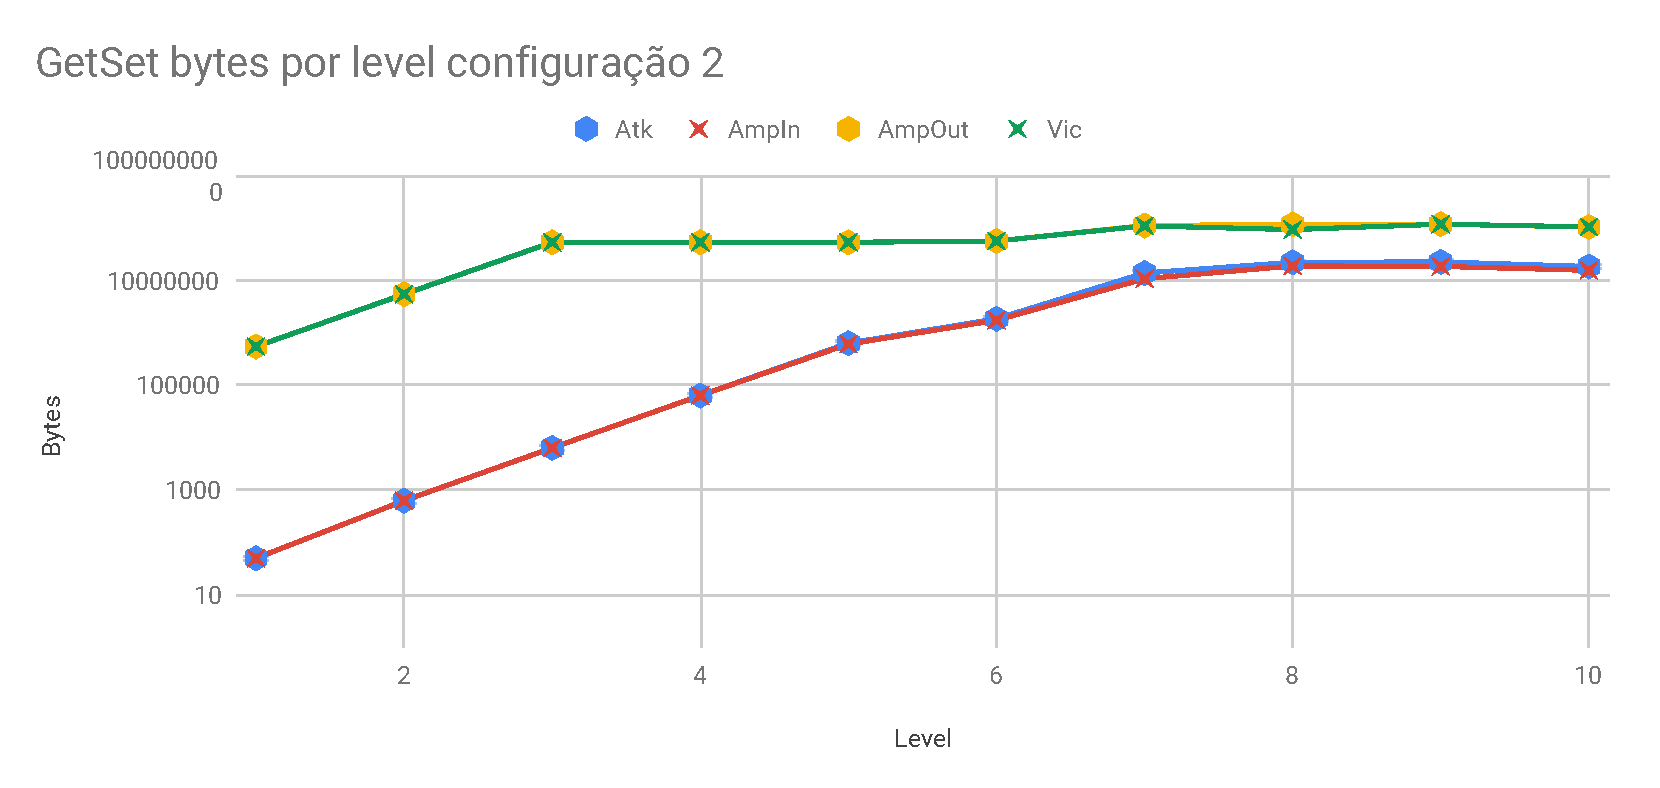
\includegraphics[scale=0.6]{img/capturas/GetSetBLC2.pdf}\
     \caption{GetSet bytes por level configuração 2}
\end{figure}

\begin{figure}[H]
     \centering
     \label{graf:GetSetFrames2}
     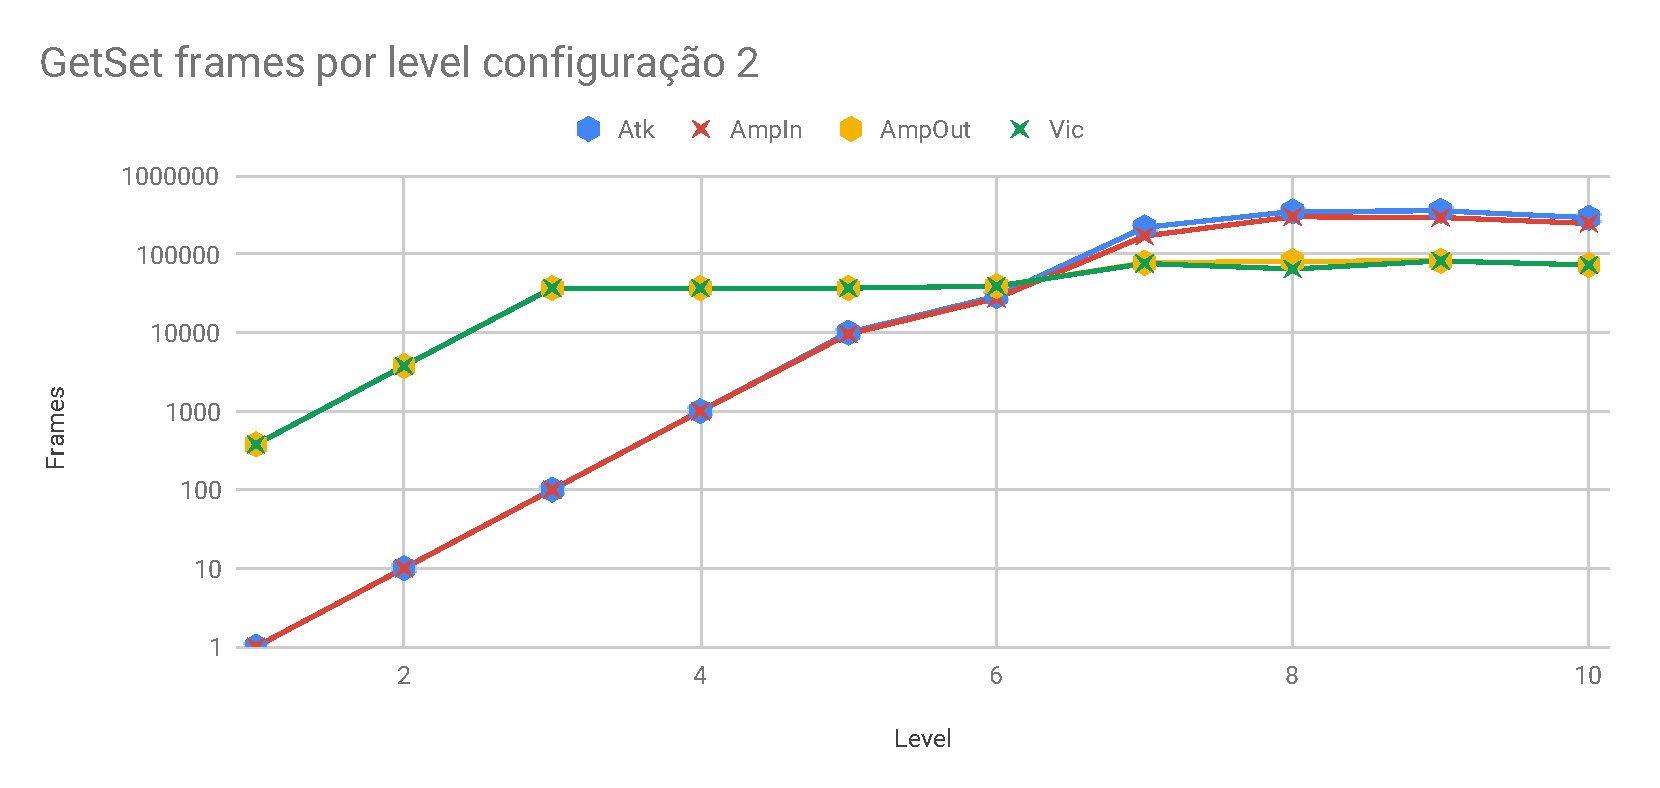
\includegraphics[scale=0.6]{img/capturas/GetSetFLC2.pdf}\
     \caption{GetSet frames por level configuração 2}
\end{figure}

\begin{table}[H]
\centering
\label{tab:bytespacsGetSet2}
\caption{Razão de bytes por pacotes para cada nível no método GetSet configuração 2}
\begin{tabular}{|c|c|c|}
\hline
Nível & Input & Output  \\ \hline
1     & 49.0  & 1440.75 \\ \hline
2     & 61.6  & 1440.78 \\ \hline
3     & 62.86 & 1440.78 \\ \hline
4     & 62.99 & 1440.78 \\ \hline
5     & 63.0  & 1440.78 \\ \hline
6     & 63.0  & 1440.79 \\ \hline
7     & 63.0  & 1440.8  \\ \hline
8     & 63.0  & 1440.8  \\ \hline
9     & 63.0  & 1440.79 \\ \hline
10    & 63.0  & 1440.79 \\ \hline
\end{tabular}
\end{table}

\subsubsection{Stats}

\begin{figure}[H]
     \centering
     \label{graf:StatsBytes2}
     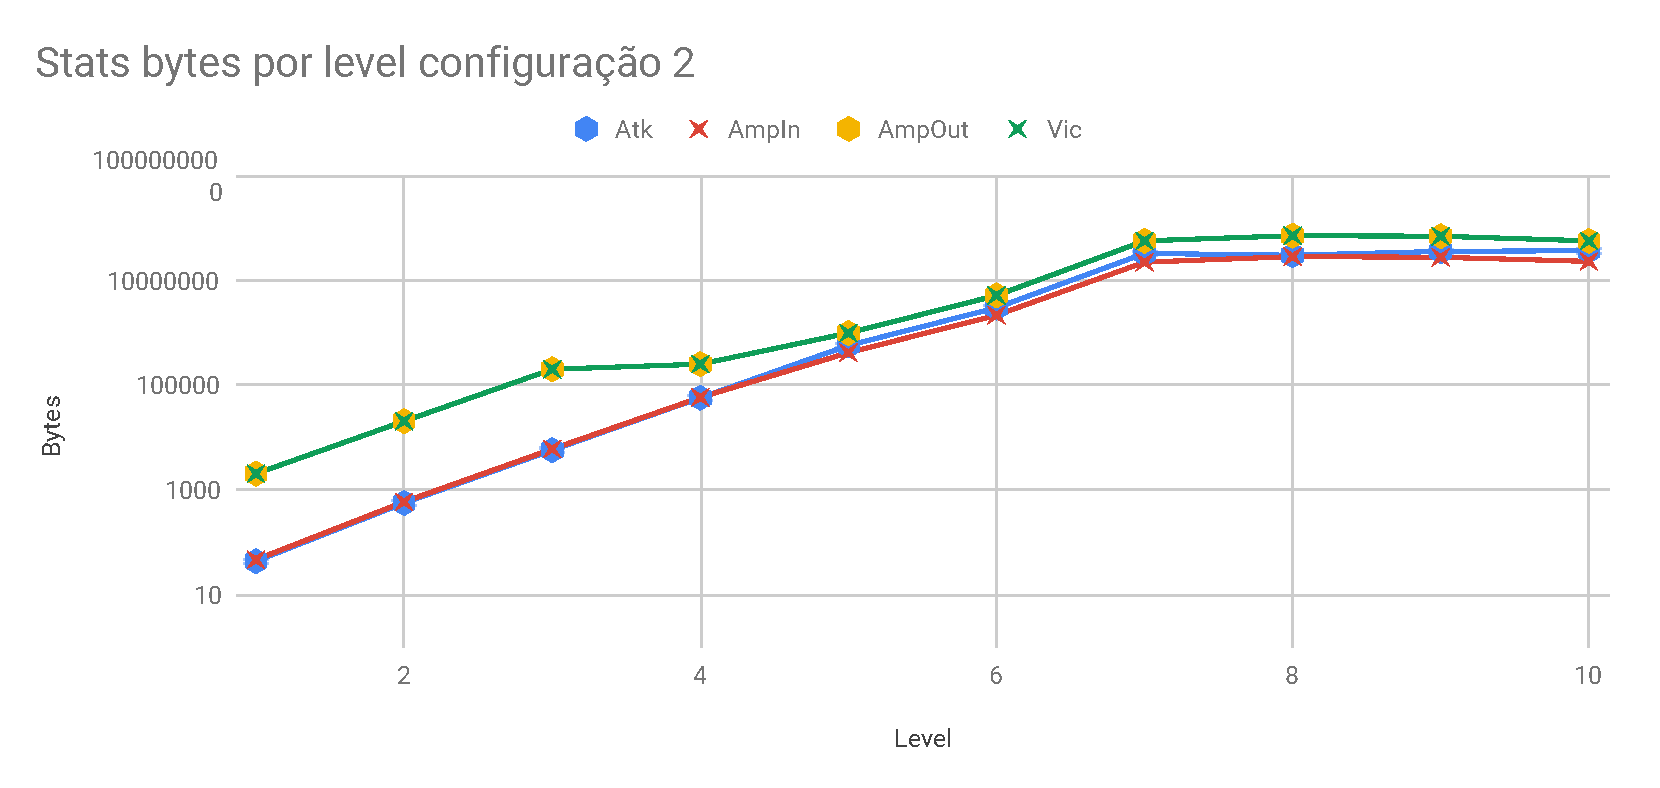
\includegraphics[scale=0.6]{img/capturas/StatsBLC2.pdf}\
     \caption{Stats bytes por level configuração 2}
\end{figure}

\begin{figure}[H]
     \centering
     \label{graf:StatsFrames2}
     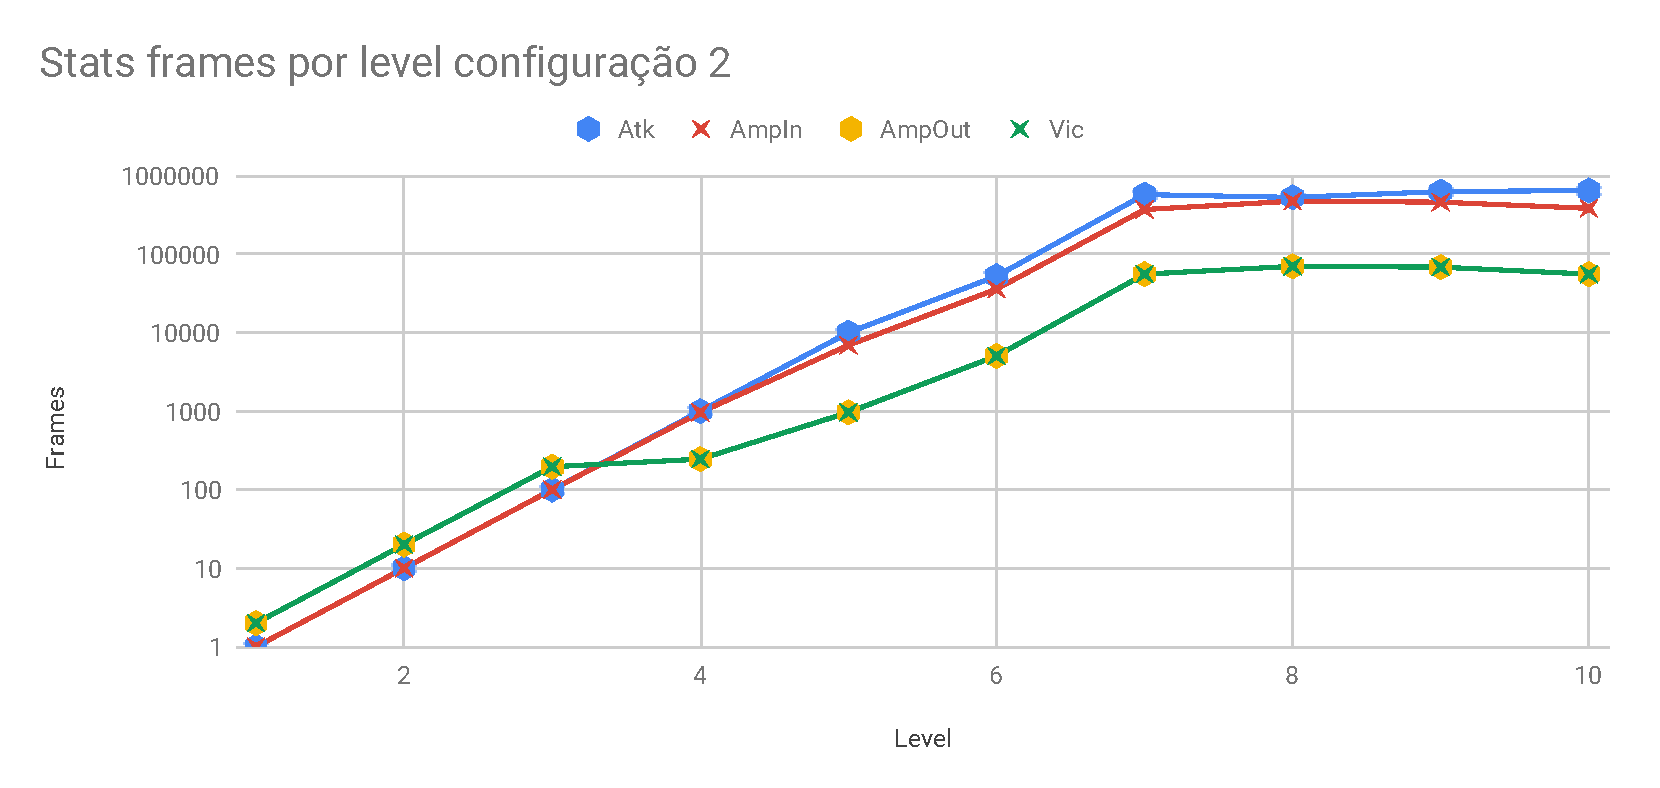
\includegraphics[scale=0.6]{img/capturas/StatsFLC2.pdf}\
     \caption{Stats frames por level configuração 2}
\end{figure}

\begin{table}[H]
\centering
\label{tab:bytespacsStats2}
\caption{Razão de bytes por pacotes para cada nível no método Stats configuração 2}
\begin{tabular}{|c|c|c|}
\hline
Nível & Input & Output  \\ \hline
1     & 46.0  & 1011.5  \\ \hline
2     & 58.6  & 1017.8  \\ \hline
3     & 59.86 & 1018.43 \\ \hline
4     & 60.04 & 1020.93 \\ \hline
5     & 60.0  & 1018.7  \\ \hline
6     & 60.0  & 1018.5  \\ \hline
7     & 60.0  & 1018.51 \\ \hline
8     & 60.0  & 1018.51 \\ \hline
9     & 60.0  & 1018.63 \\ \hline
10    & 60.0  & 1019.01 \\ \hline
\end{tabular}
\end{table}

\subsection*{Configuração 3}

Essa configuração se caracteriza por ter o atacante e vítima mais fortes e o refletor mais
fraco.

No método GetSet tivemos um máximo de 63 bytes/pacotes chegando no amplificador no nível 5 e um máximo de 1440.8 bytes/pacotes saindo do amplificador no nível 7 como apresentado na tabela \ref{tab:bytespacsGetSet3}, com o atacante saturando no nível 7 como mostra os gráficos \ref{graf:GetSetBytes3} e \ref{graf:GetSetFrames3}.

Já para o método Stats tivemos um máximo de 60 bytes/pacotes chegando no amplificador no nível 5 e um máximo de 1014.53 bytes/pacotes saindo do amplificador também no nível 9 como apresentado na tabela \ref{tab:bytespacsStats3}, apesar do atacante saturar apenas no nível 7 como mostra os gráficos \ref{graf:StatsBytes3} e \ref{graf:StatsFrames3}.

\begin{table}[H]
\centering
\caption{Configuração 3}
\begin{tabular}{|l|l|}
\hline
Atacante     & Orion    \\ \hline
Refletor     & Sputnik  \\ \hline
Vítima       & Spitfire \\ \hline
\end{tabular}
\end{table}

\subsubsection{GetSet}

\begin{figure}[H]
     \centering
     \label{graf:GetSetBytes3}
     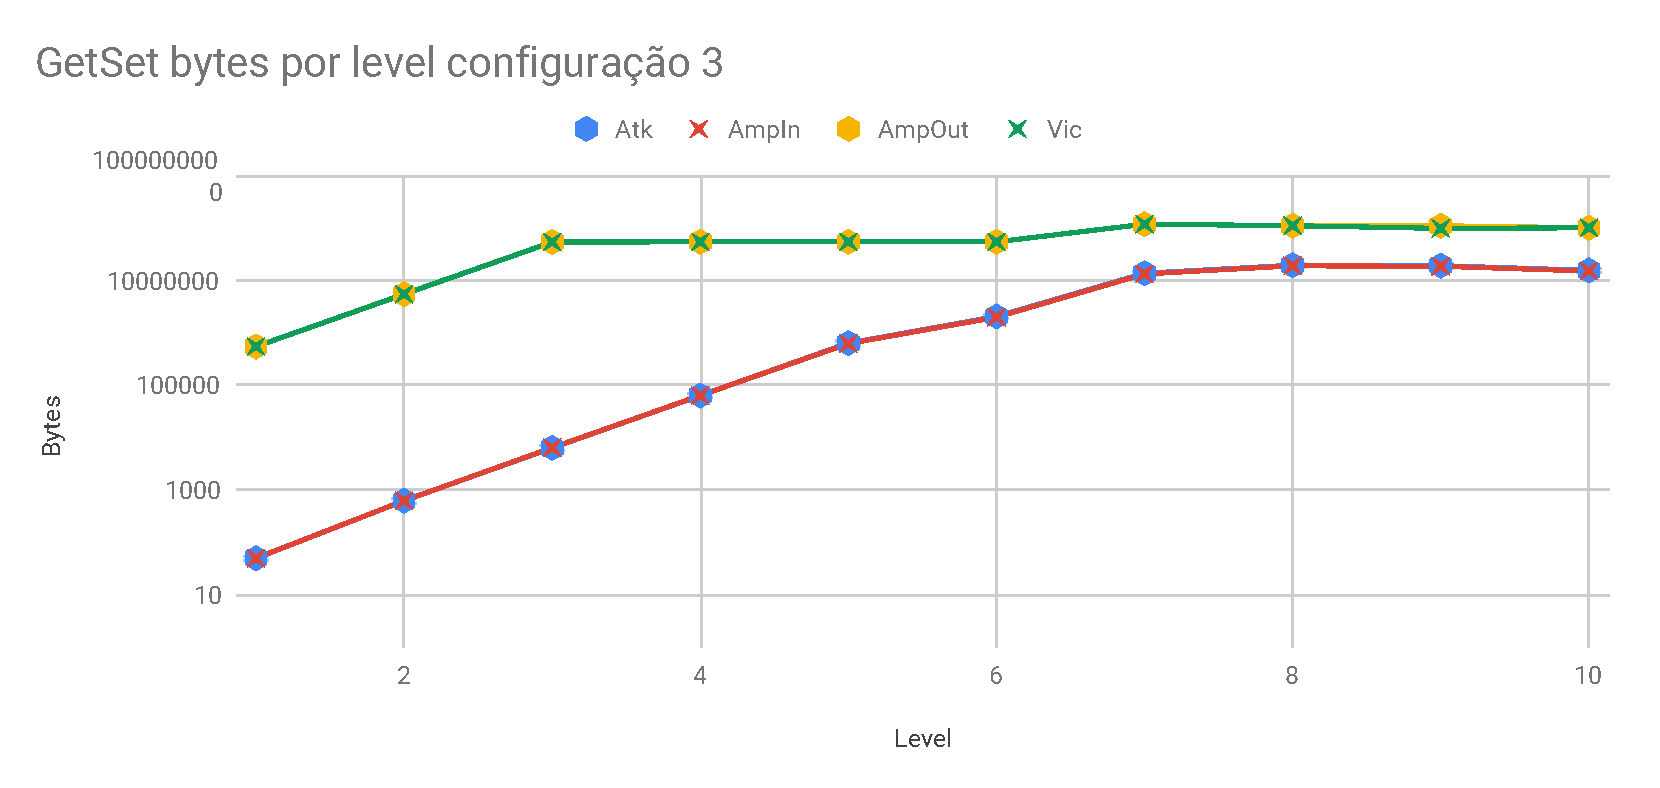
\includegraphics[scale=0.6]{img/capturas/GetSetBLC3.pdf}\
     \caption{GetSet bytes por level configuração 3}
\end{figure}

\begin{figure}[H]
     \centering
     \label{graf:GetSetFrames3}
     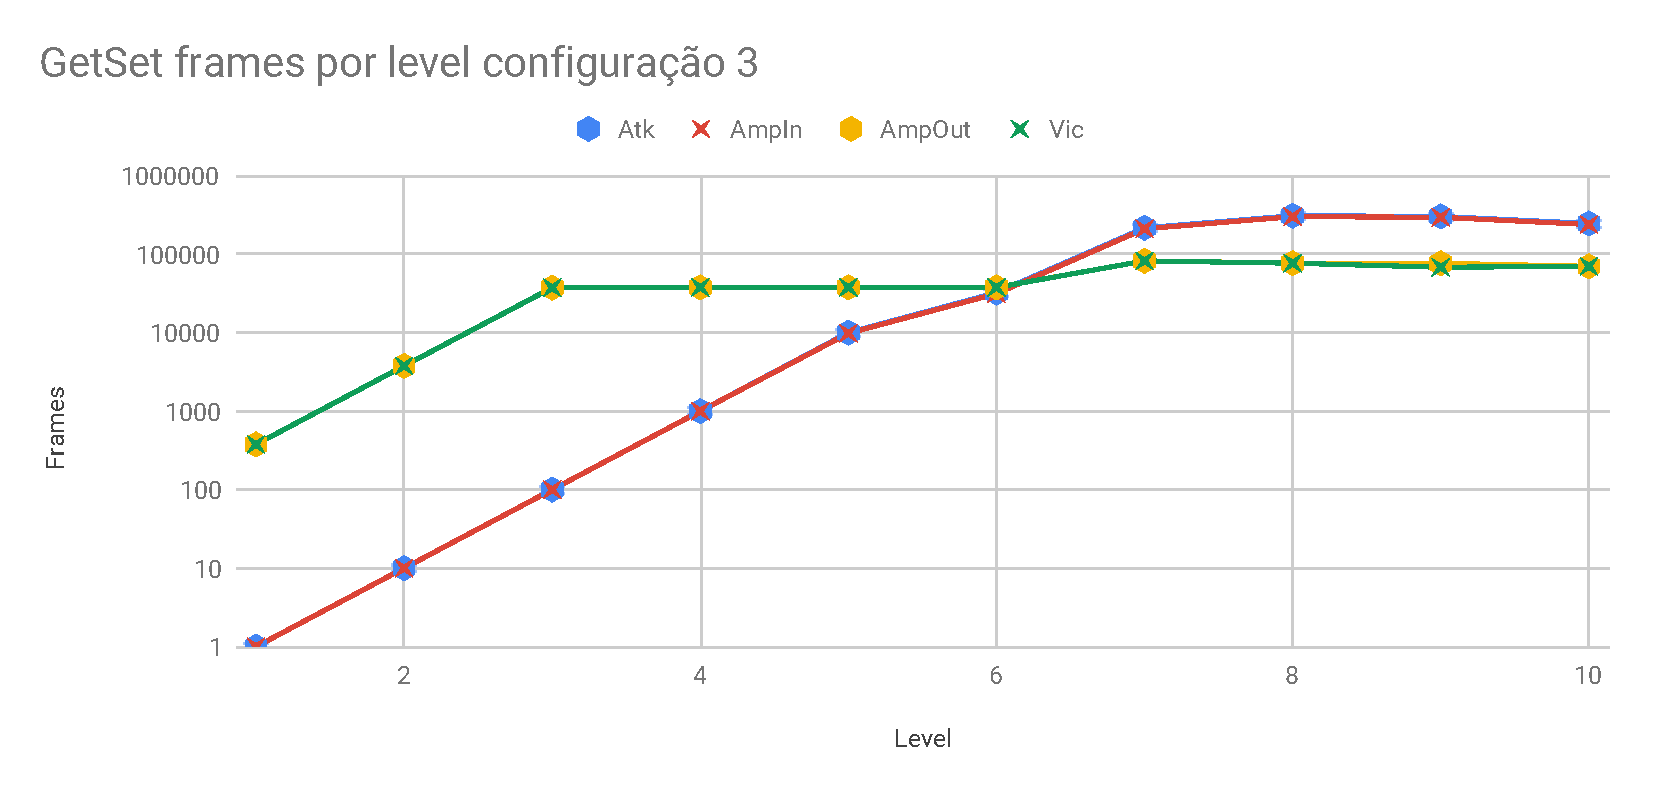
\includegraphics[scale=0.6]{img/capturas/GetSetFLC3.pdf}\
     \caption{GetSet frames por level configuração 3}
\end{figure}

\begin{table}[H]
\centering
\label{tab:bytespacsGetSet3}
\caption{Razão de bytes por pacotes para cada nível no método GetSet configuração 3}
\begin{tabular}{|c|c|c|}
\hline
Nível & Input & Output  \\ \hline
1     & 49.0  & 1440.75 \\ \hline
2     & 61.6  & 1440.78 \\ \hline
3     & 63.23 & 1440.78 \\ \hline
4     & 62.99 & 1440.78 \\ \hline
5     & 63.0  & 1440.78 \\ \hline
6     & 63.0  & 1440.78 \\ \hline
7     & 63.0  & 1440.8  \\ \hline
8     & 63.0  & 1440.78 \\ \hline
9     & 63.0  & 1440.8  \\ \hline
10    & 63.0  & 1440.78 \\ \hline
\end{tabular}
\end{table}

\subsubsection{Stats}

\begin{figure}[H]
     \centering
     \label{graf:StatsBytes3}
     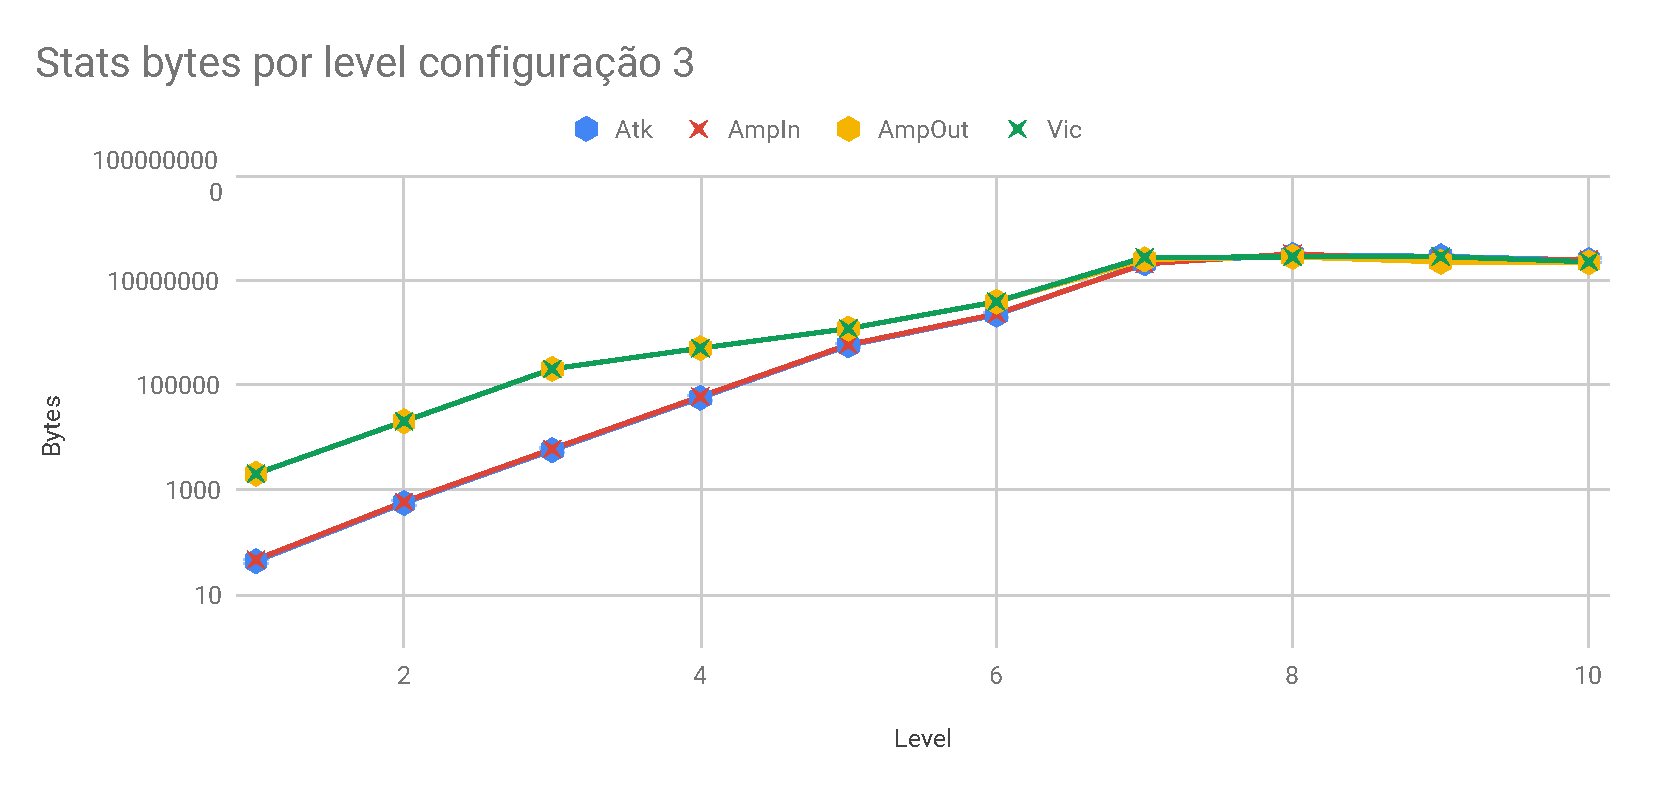
\includegraphics[scale=0.6]{img/capturas/StatsBLC3.pdf}\
     \caption{Stats bytes por level configuração 3}
\end{figure}

\begin{figure}[H]
     \centering
     \label{graf:StatsFrames3}
     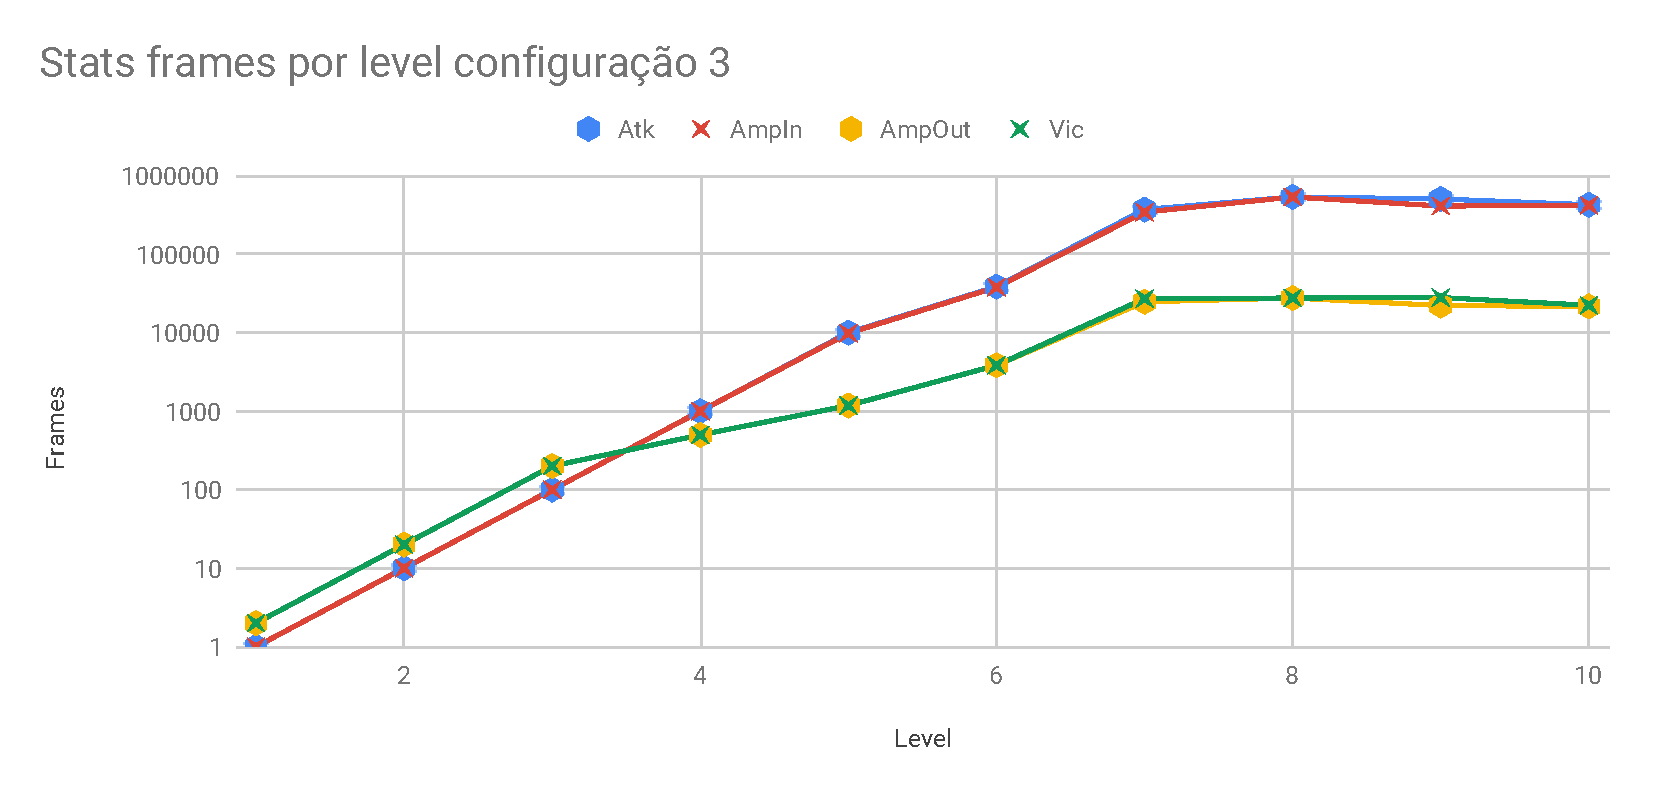
\includegraphics[scale=0.6]{img/capturas/StatsFLC3.pdf}\
     \caption{Stats frames por level configuração 3}
\end{figure}

\begin{table}[H]
\centering
\label{tab:bytespacsStats3}
\caption{Razão de bytes por pacotes para cada nível no método Stats configuração 3}
\begin{tabular}{|c|c|c|}
\hline
Nível & Input & Output  \\ \hline
1     & 46.0  & 1007.0  \\ \hline
2     & 58.6  & 1013.3  \\ \hline
3     & 59.86 & 1013.93 \\ \hline
4     & 59.99 & 1013.97 \\ \hline
5     & 60.0  & 1013.99 \\ \hline
6     & 60.0  & 1014.0  \\ \hline
7     & 60.0  & 1014.02 \\ \hline
8     & 60.0  & 1014.29 \\ \hline
9     & 60.0  & 1014.53 \\ \hline
10    & 60.0  & 1014.52 \\ \hline
\end{tabular}
\end{table}

\subsection*{Configuração 4}

Essa configuração se caracteriza por ter o refletor e vítima mais fortes e a atacante
mais fraco, similar a configuração 1.

No método GetSet tivemos um máximo de 63 bytes/pacotes chegando no amplificador no nível 5 e um máximo de 1440.99 bytes/pacotes saindo do amplificador no nível 1 como apresentado na tabela \ref{tab:bytespacsGetSet4}, apesar do atacante saturar apenas no nível 7 como mostra os gráficos \ref{graf:GetSetBytes4} e \ref{graf:GetSetFrames4}.

Já para o método Stats tivemos um máximo de 60.01 bytes/pacotes chegando no amplificador no nível 5 e um máximo de 1905 bytes/pacotes saindo do amplificador também no nível 1 como apresentado na tabela \ref{tab:bytespacsStats4}, apesar do atacante saturar apenas no nível 7 como mostra os gráficos \ref{graf:StatsBytes4} e \ref{graf:StatsFrames4}.

\begin{table}[H]
\centering
\caption{Configuração 4}
\begin{tabular}{|l|l|}
\hline
Atacante     & Sputnik  \\ \hline
Amplificador & Orion    \\ \hline
Vítima       & Spitfire \\ \hline
\end{tabular}
\end{table}

\subsubsection{GetSet}

\begin{figure}[H]
     \centering
     \label{graf:GetSetBytes4}
     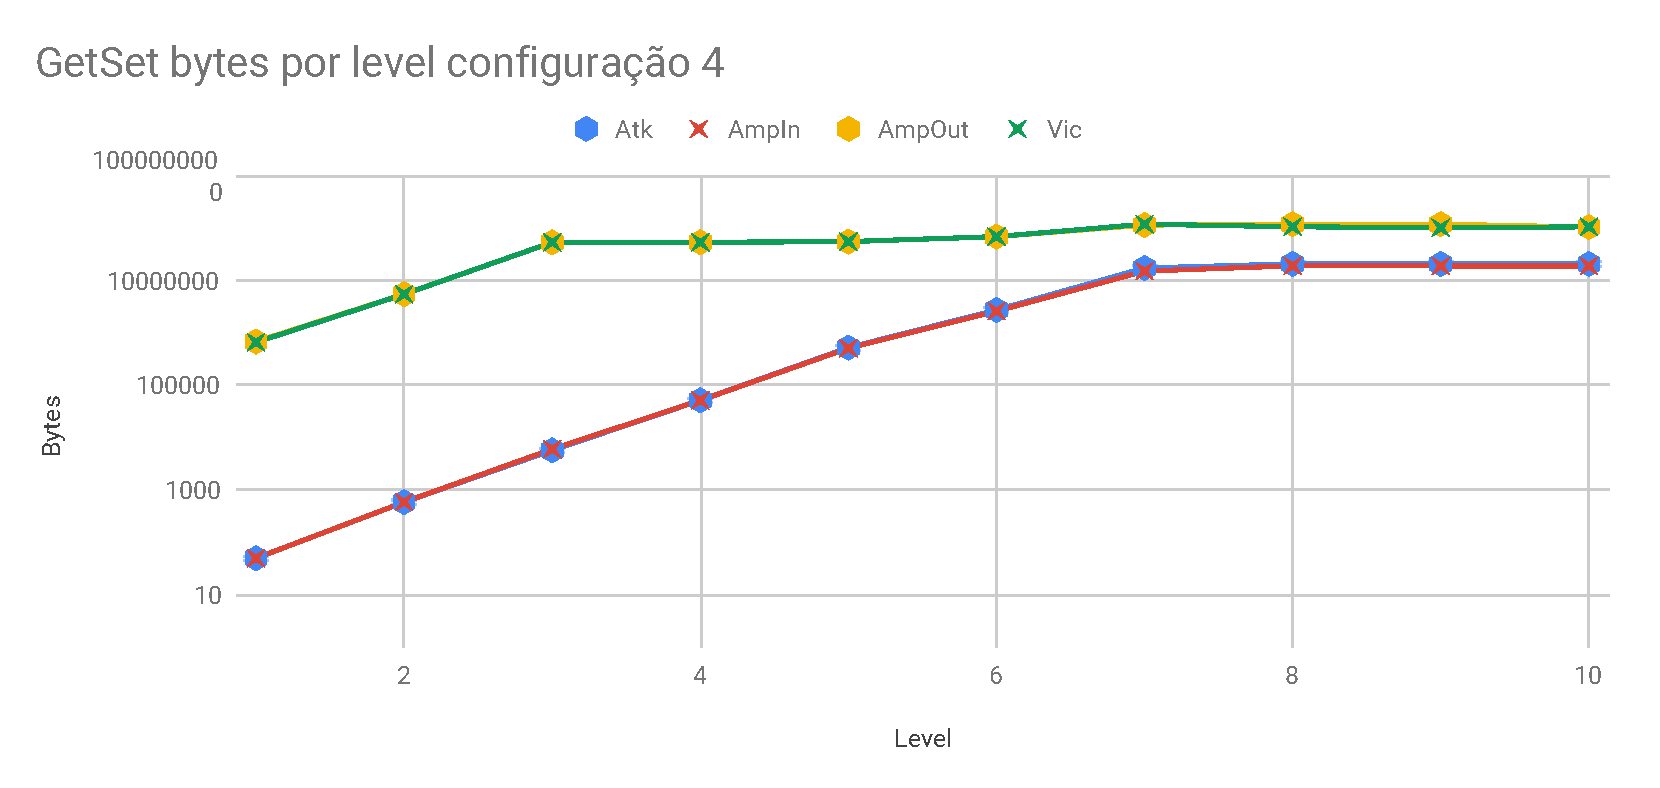
\includegraphics[scale=0.6]{img/capturas/GetSetBLC4.pdf}\
     \caption{GetSet bytes por level configuração 4}
\end{figure}

\begin{figure}[H]
     \centering
     \label{graf:GetSetFrames4}
     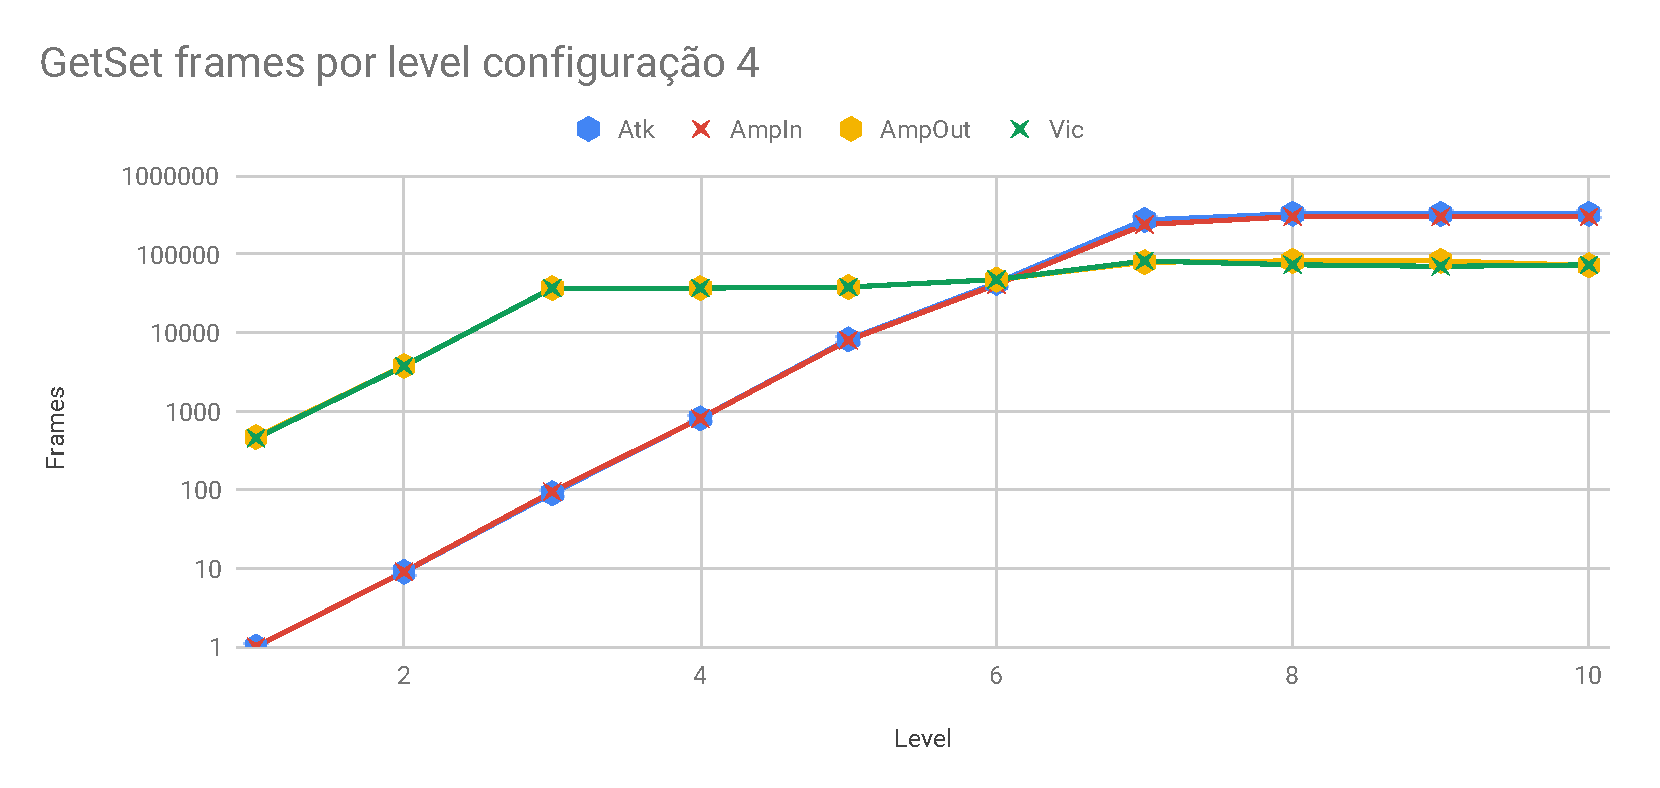
\includegraphics[scale=0.6]{img/capturas/GetSetFLC4.pdf}\
     \caption{GetSet frames por level configuração 4}
\end{figure}

\begin{table}[H]
\centering
\label{tab:bytespacsGetSet4}
\caption{Razão de bytes por pacotes para cada nível no método GetSet configuração 4}
\begin{tabular}{|c|c|c|}
\hline
Nível & Input & Output  \\ \hline
1     & 49.0  & 1440.99 \\ \hline
2     & 64.22 & 1440.93 \\ \hline
3     & 63.24 & 1440.81 \\ \hline
4     & 62.98 & 1440.78 \\ \hline
5     & 63.0  & 1440.78 \\ \hline
6     & 63.0  & 1440.8  \\ \hline
7     & 63.0  & 1440.8  \\ \hline
8     & 63.0  & 1440.78 \\ \hline
9     & 63.0  & 1440.78 \\ \hline
10    & 63.0  & 1440.78 \\ \hline
\end{tabular}
\end{table}

\subsubsection{Stats}

\begin{figure}[H]
     \centering
     \label{graf:StatsBytes4}
     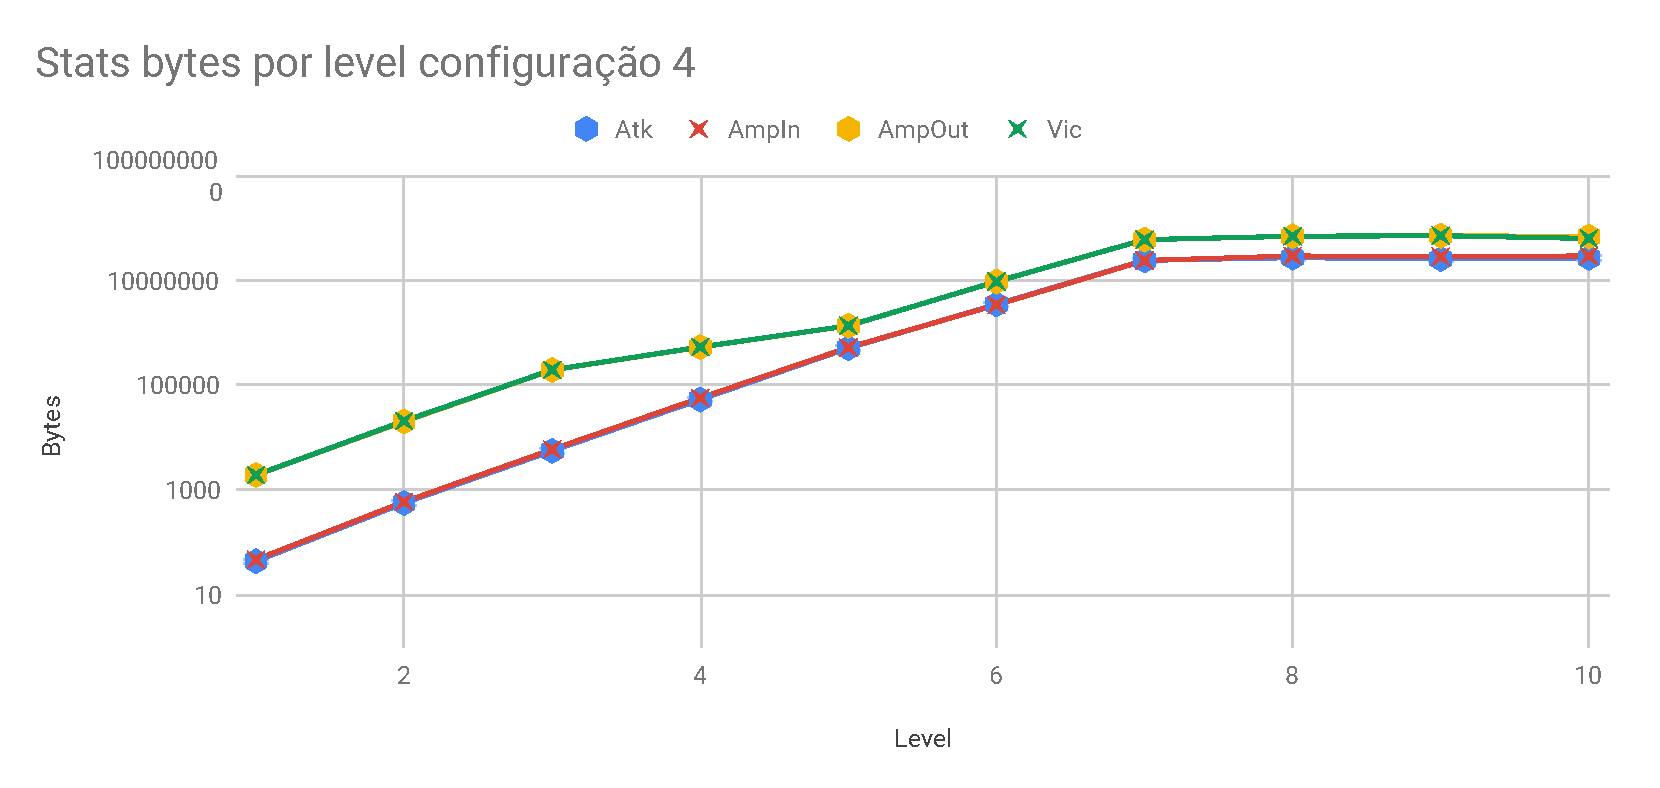
\includegraphics[scale=0.6]{img/capturas/StatsBLC4.pdf}\
     \caption{Stats bytes por level configuração 4}
\end{figure}

\begin{figure}[H]
     \centering
     \label{graf:StatsFrames4}
     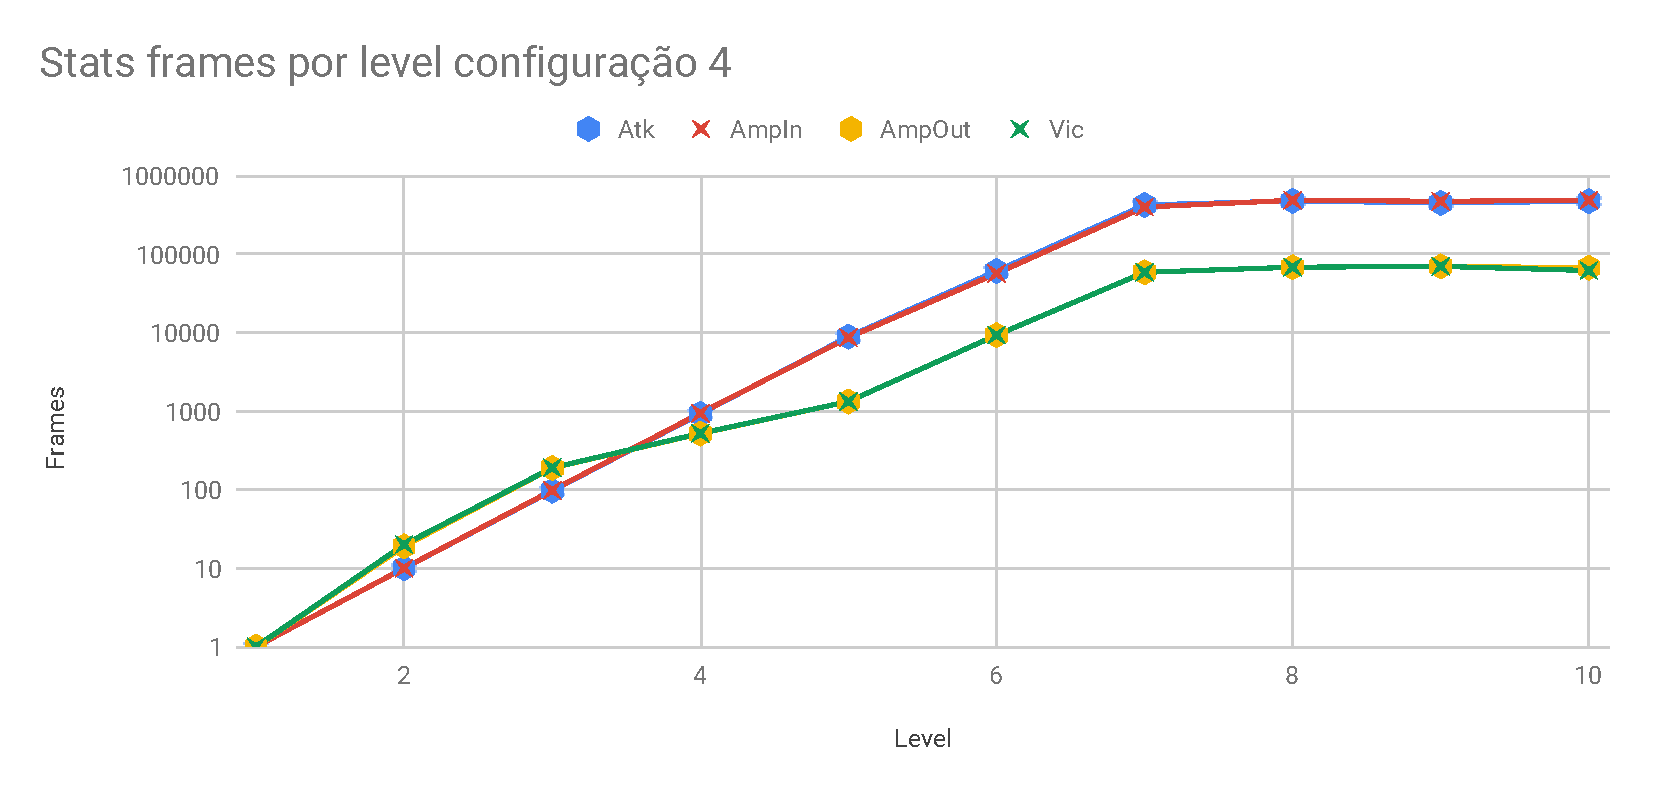
\includegraphics[scale=0.6]{img/capturas/StatsFLC4.pdf}\
     \caption{Stats frames por level configuração 4}
\end{figure}

\begin{table}[H]
\centering
\label{tab:bytespacsStats4}
\caption{Razão de bytes por pacotes para cada nível no método Stats configuração 4}
\begin{tabular}{|c|c|c|}
\hline
Nível & Input & Output  \\ \hline
1     & 46.0  & 1905.0  \\ \hline
2     & 58.6  & 1057.21 \\ \hline
3     & 59.86 & 1024.19 \\ \hline
4     & 60.0  & 1020.49 \\ \hline
5     & 60.01 & 1019.95 \\ \hline
6     & 60.0  & 1019.54 \\ \hline
7     & 60.0  & 1019.51 \\ \hline
8     & 60.0  & 1019.5  \\ \hline
9     & 60.0  & 1019.51 \\ \hline
10    & 60.0  & 1019.51 \\ \hline
\end{tabular}
\end{table}

\subsection*{Configuração 5}

Essa configuração se caracteriza por ter o atacante e vítima mais fortes e a vítima
mais fraca, similar a configuração 3.

No método GetSet tivemos um máximo de 63 bytes/pacotes chegando no amplificador no nível 5 e um máximo de 1440.8 bytes/pacotes saindo do amplificador no nível 8 como apresentado na tabela \ref{tab:bytespacsGetSet5}, apesar do atacante saturar apenas no nível 8 como mostra os gráficos \ref{graf:GetSetBytes5} e \ref{graf:GetSetFrames5}.

Já para o método Stats tivemos um máximo de 60 bytes/pacotes chegando no amplificador no nível 5 e um máximo de 1018.18 bytes/pacotes saindo do amplificador também no nível 10 como apresentado na tabela \ref{tab:bytespacsStats5}, com o atacante saturando no nível 7 como mostra os gráficos \ref{graf:StatsBytes5} e \ref{graf:StatsFrames5}.

\begin{table}[H]
\centering
\caption{Configuração 5}
\begin{tabular}{|l|l|}
\hline
Atacante     & Spitfire \\ \hline
Amplificador & Sputnik  \\ \hline
Vítima       & Orion    \\ \hline
\end{tabular}
\end{table}

\subsubsection{GetSet}

\begin{figure}[H]
     \centering
     \label{graf:GetSetBytes5}
     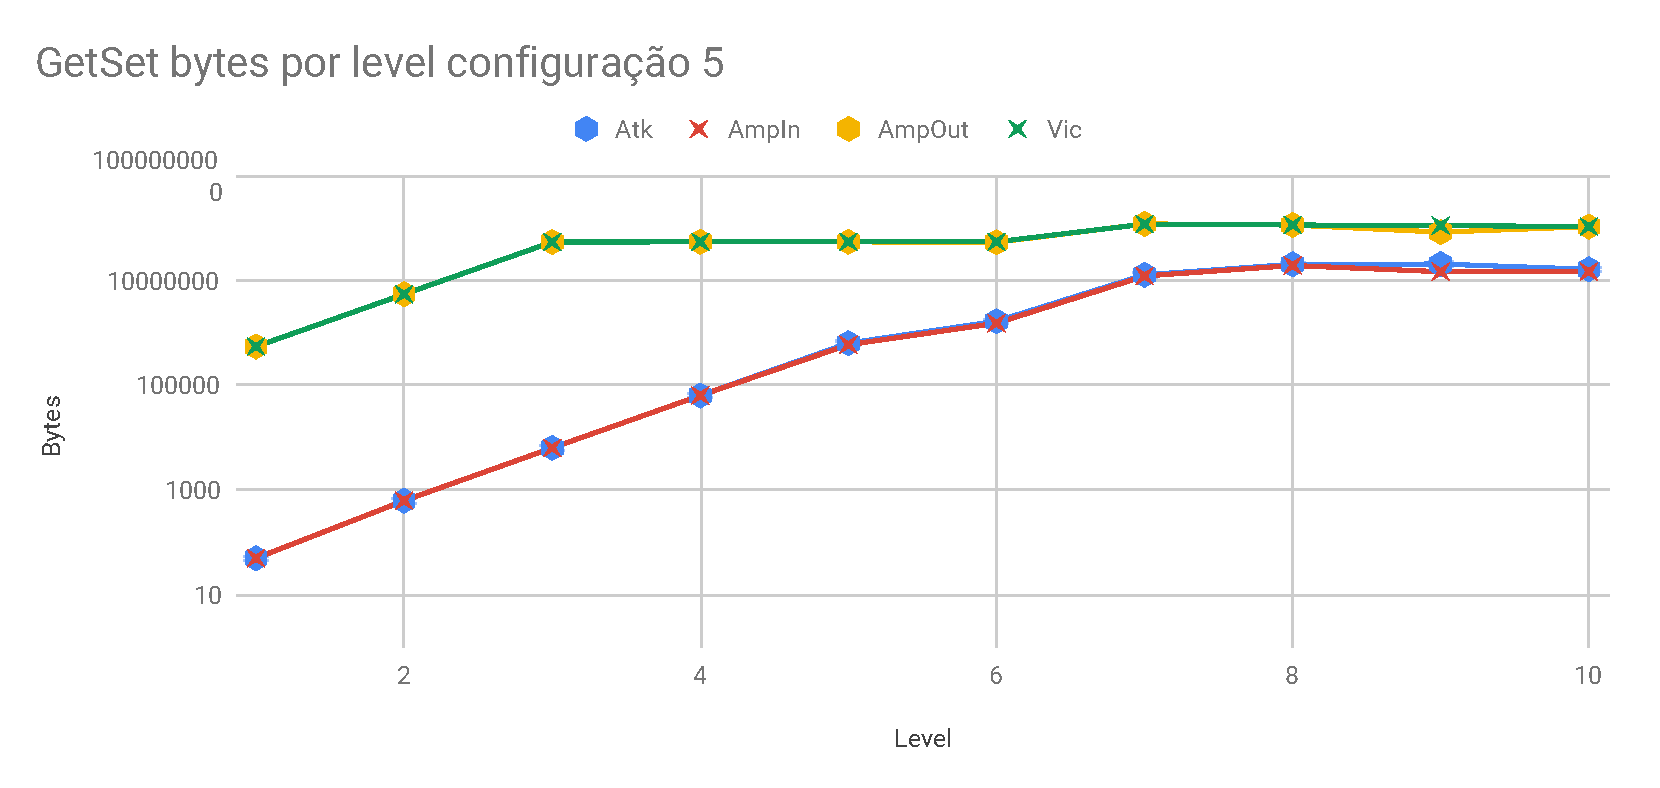
\includegraphics[scale=0.6]{img/capturas/GetSetBLC5.pdf}\
     \caption{GetSet bytes por level configuração 5}
\end{figure}

\begin{figure}[H]
     \centering
     \label{graf:GetSetFrames5}
     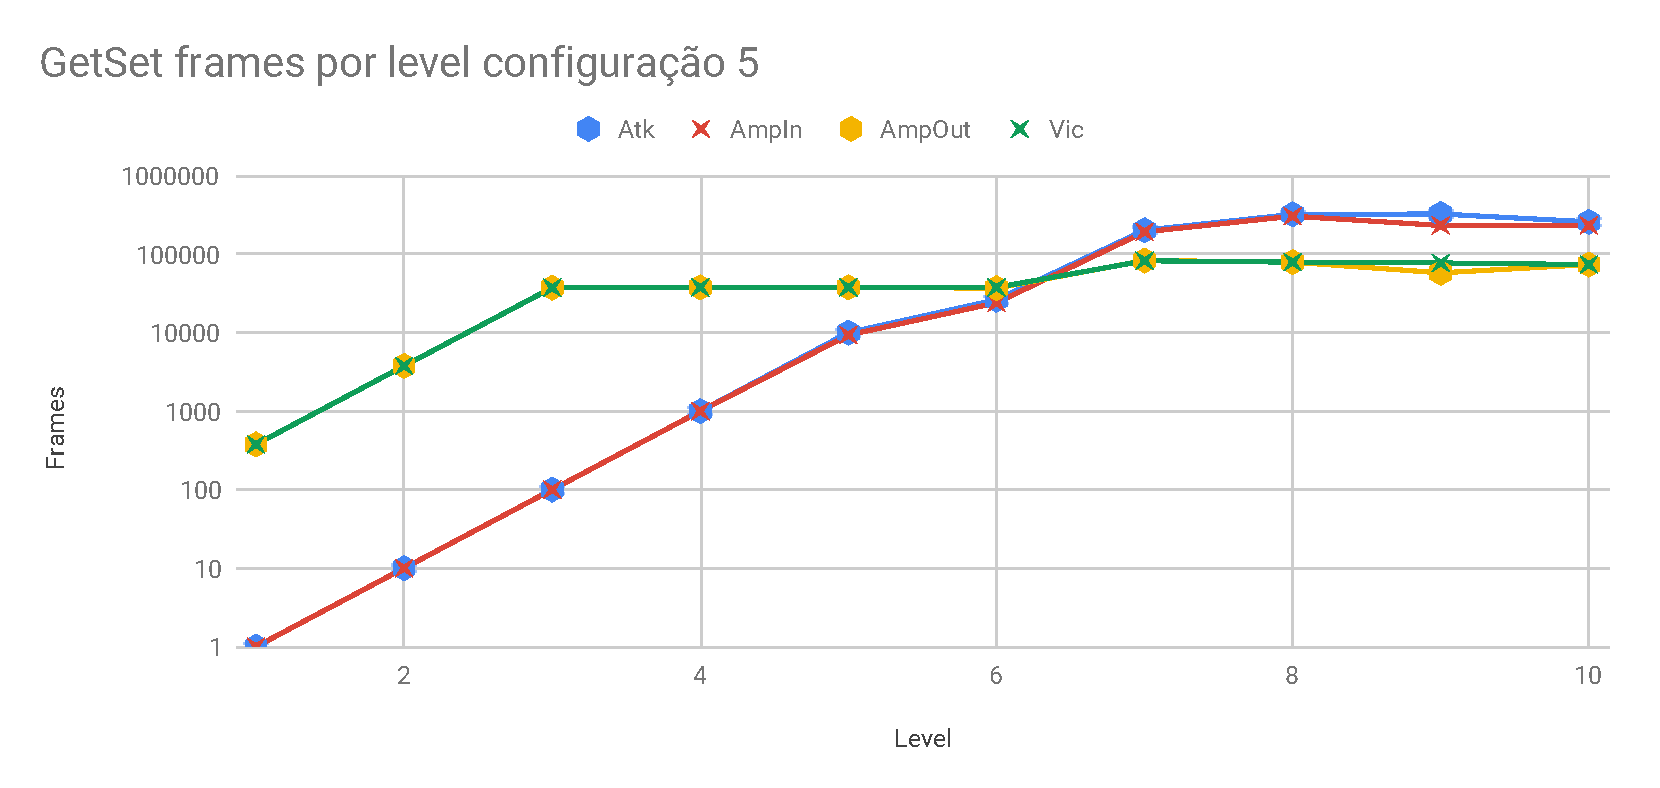
\includegraphics[scale=0.6]{img/capturas/GetSetFLC5.pdf}\
     \caption{GetSet frames por level configuração 5}
\end{figure}

\begin{table}[H]
\centering
\label{tab:bytespacsGetSet5}
\caption{Razão de bytes por pacotes para cada nível no método GetSet configuração 5}
\begin{tabular}{|c|c|c|}
\hline
Nível & Input & Output  \\ \hline
1     & 49.0  & 1440.75 \\ \hline
2     & 61.6  & 1440.78 \\ \hline
3     & 62.86 & 1440.78 \\ \hline
4     & 62.99 & 1440.78 \\ \hline
5     & 63.0  & 1440.78 \\ \hline
6     & 63.0  & 1440.79 \\ \hline
7     & 63.0  & 1440.78 \\ \hline
8     & 63.0  & 1440.8  \\ \hline
9     & 63.0  & 1440.78 \\ \hline
10    & 63.0  & 1440.79 \\ \hline
\end{tabular}
\end{table}

\subsubsection{Stats}

\begin{figure}[H]
     \centering
     \label{graf:StatsBytes5}
     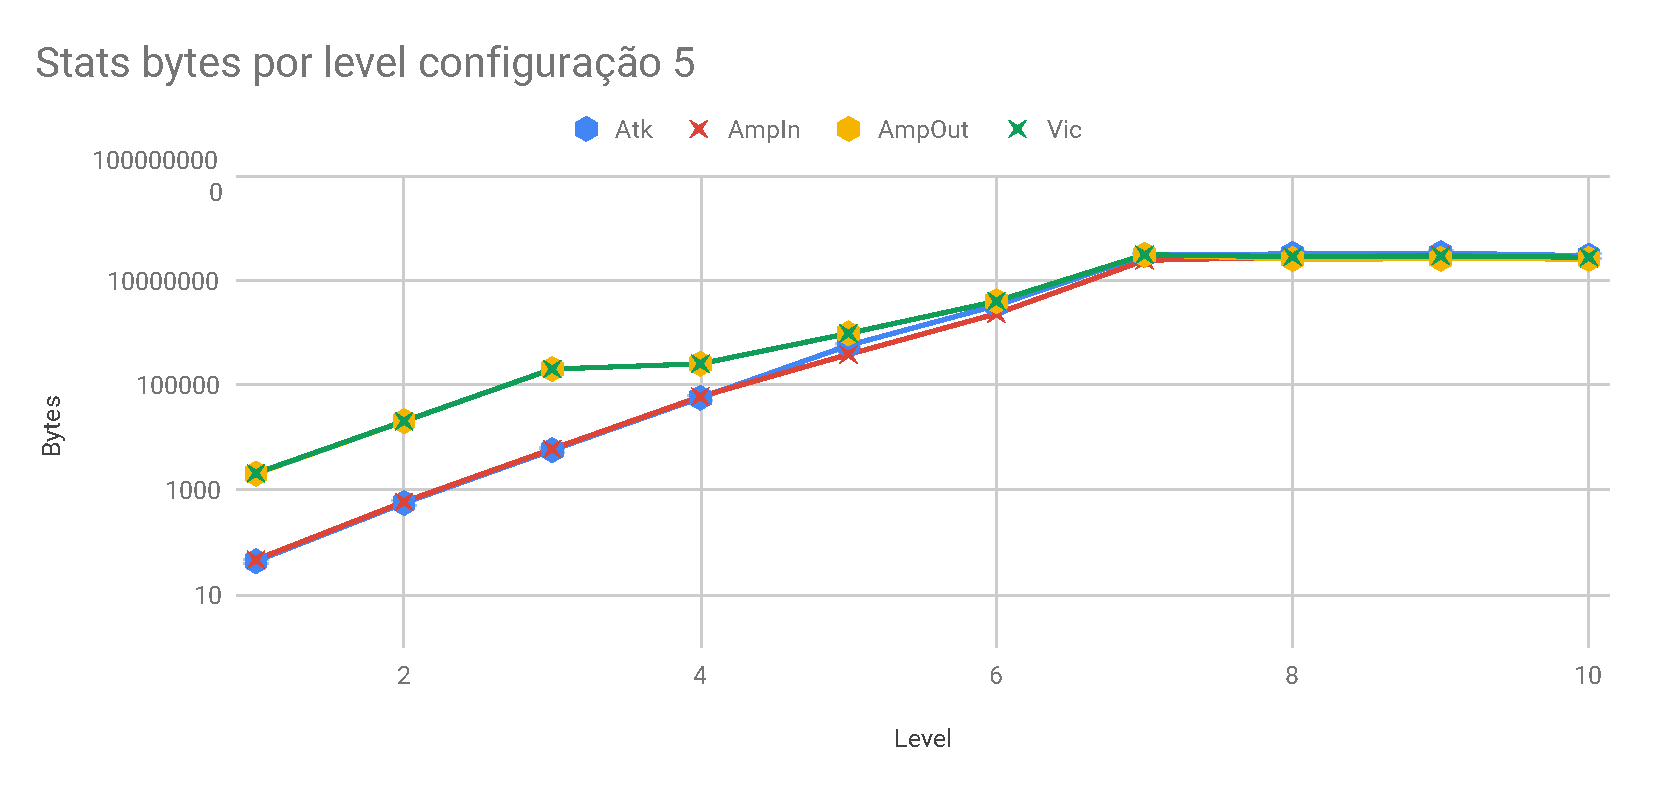
\includegraphics[scale=0.6]{img/capturas/StatsBLC5.pdf}\
     \caption{Stats bytes por level configuração 5}
\end{figure}

\begin{figure}[H]
     \centering
     \label{graf:StatsFrames5}
     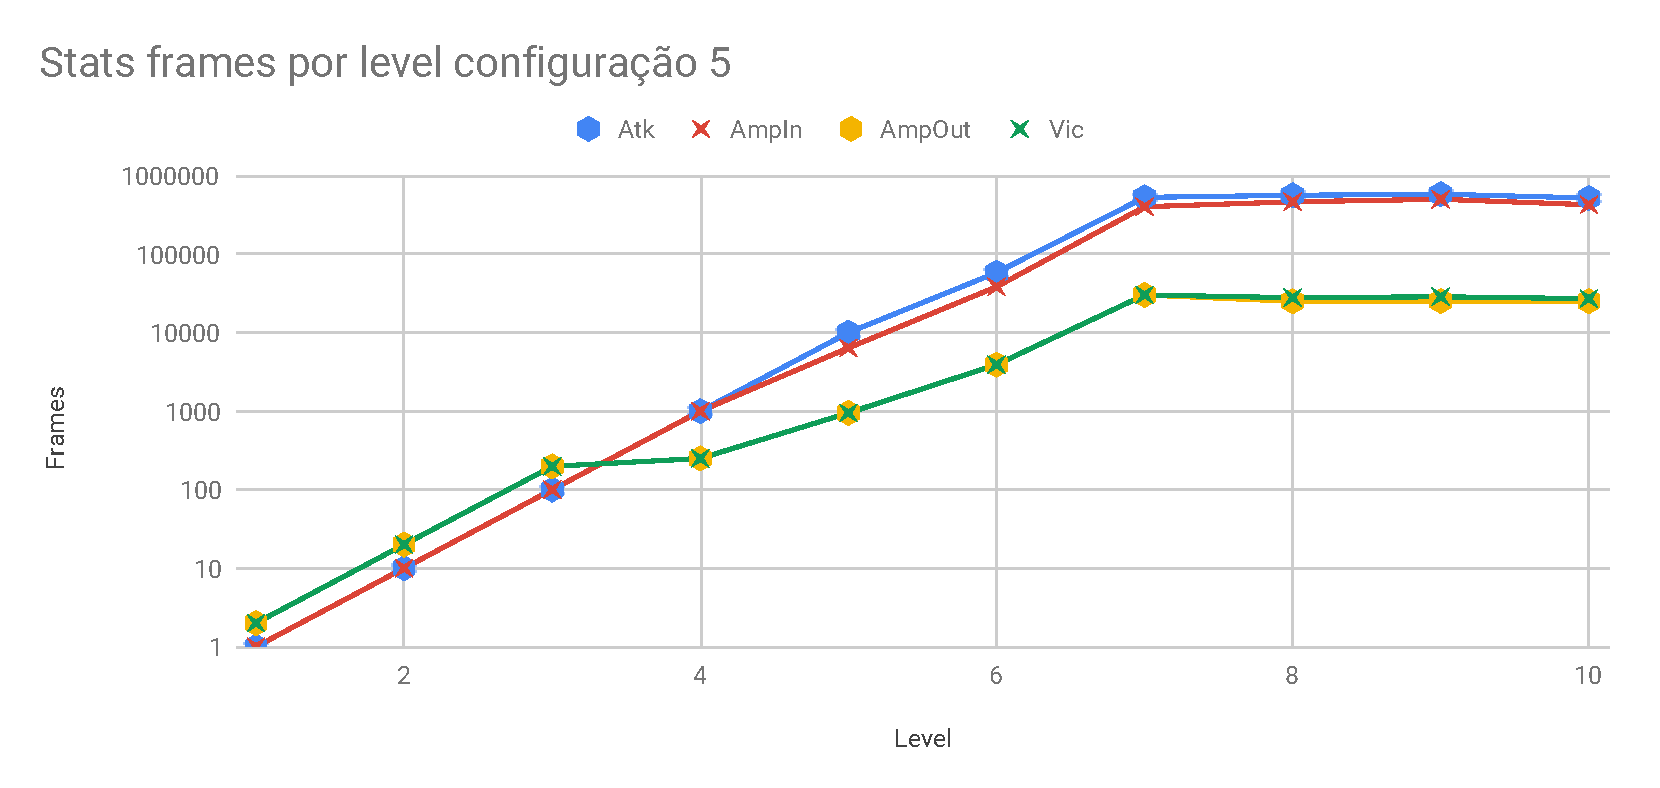
\includegraphics[scale=0.6]{img/capturas/StatsFLC5.pdf}\
     \caption{Stats frames por level configuração 5}
\end{figure}

\begin{table}[H]
\centering
\label{tab:bytespacsStats5}
\caption{Razão de bytes por pacotes para cada nível no método Stats configuração 5}
\begin{tabular}{|c|c|c|}
\hline
Nível & Input & Output  \\ \hline
1     & 46.0  & 1010.5  \\ \hline
2     & 58.6  & 1016.8  \\ \hline
3     & 59.86 & 1017.43 \\ \hline
4     & 59.99 & 1017.44 \\ \hline
5     & 60.0  & 1017.49 \\ \hline
6     & 60.0  & 1017.5  \\ \hline
7     & 60.0  & 1017.5  \\ \hline
8     & 60.0  & 1017.53 \\ \hline
9     & 60.0  & 1017.66 \\ \hline
10    & 60.0  & 1018.18 \\ \hline
\end{tabular}
\end{table}

\subsection*{Configuração 6}

Essa configuração se caracteriza por ter o refletor e atacante mais fortes e a vítima mais
fraca, semelhante a configuração 2.

No método GetSet tivemos um máximo de 63 bytes/pacotes chegando no amplificador no nível 5 e um máximo de 1440.81 bytes/pacotes saindo do amplificador no nível 6 como apresentado na tabela \ref{tab:bytespacsGetSet6}, com o atacante saturando no nível 8 como mostra os gráficos \ref{graf:GetSetBytes6} e \ref{graf:GetSetFrames6}.

Já para o método Stats tivemos um máximo de 60 bytes/pacotes chegando no amplificador no nível 4 e um máximo de 1045.79 bytes/pacotes saindo do amplificador também no nível 2 como apresentado na tabela \ref{tab:bytespacsStats6}, apesar do atacante saturar no nível 8 como mostra os gráficos \ref{graf:StatsBytes6} e \ref{graf:StatsFrames6}.

\begin{table}[H]
\centering
\caption{Configuração 6}
\begin{tabular}{|l|l|}
\hline
Atacante     & Orion    \\ \hline
Amplificador & Spitfire \\ \hline
Vítima       & Sputnik  \\ \hline
\end{tabular}
\end{table}

\subsubsection{GetSet}

\begin{figure}[H]
     \centering
     \label{graf:GetSetBytes6}
     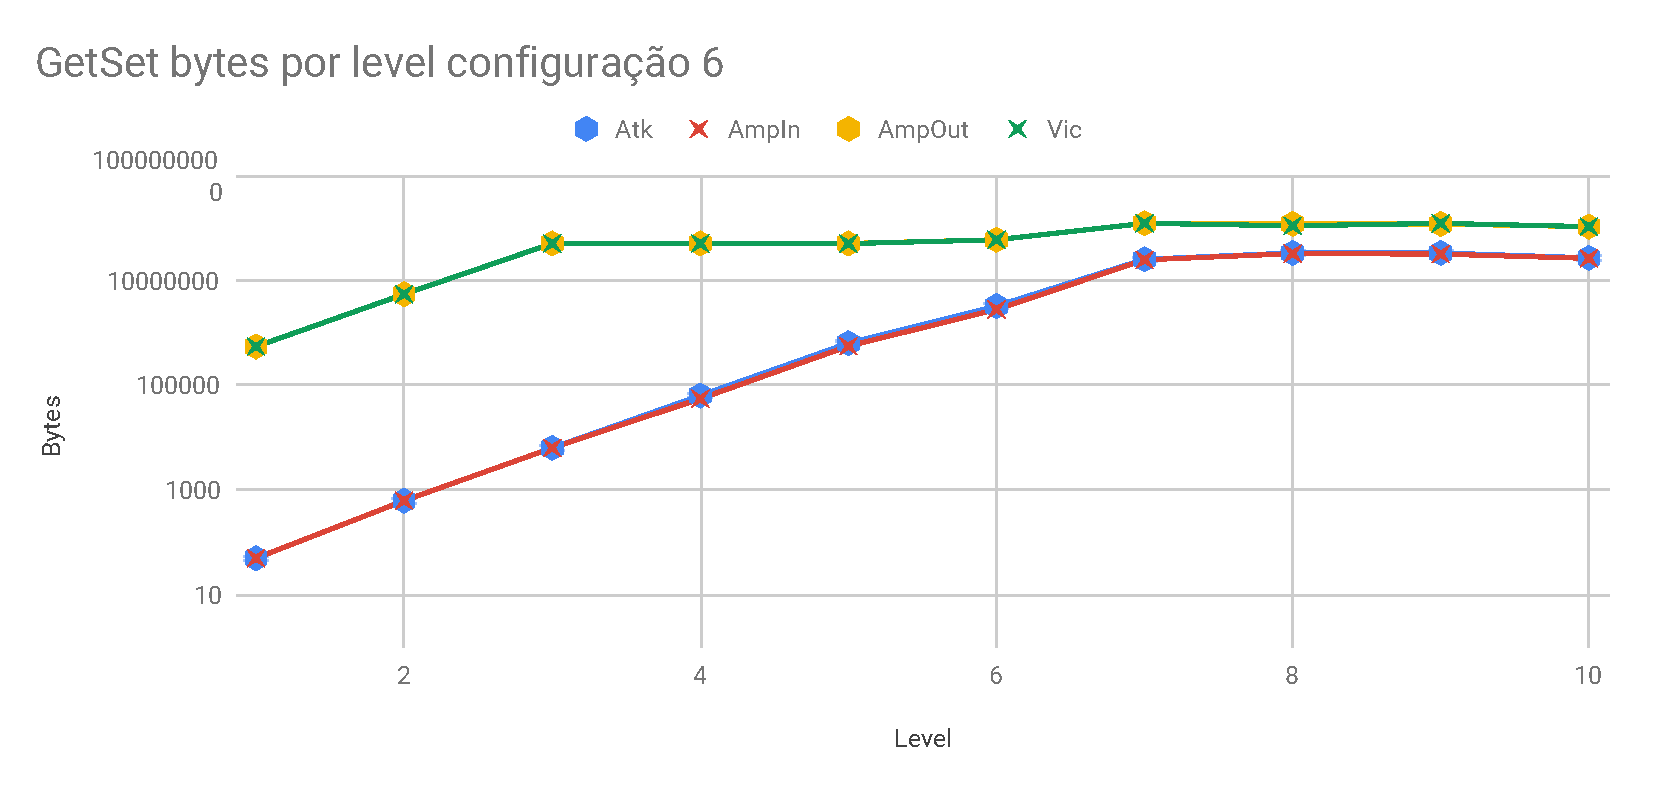
\includegraphics[scale=0.6]{img/capturas/GetSetBLC6.pdf}\
     \caption{GetSet bytes por level configuração 6}
\end{figure}

\begin{figure}[H]
     \centering
     \label{graf:GetSetFrames6}
     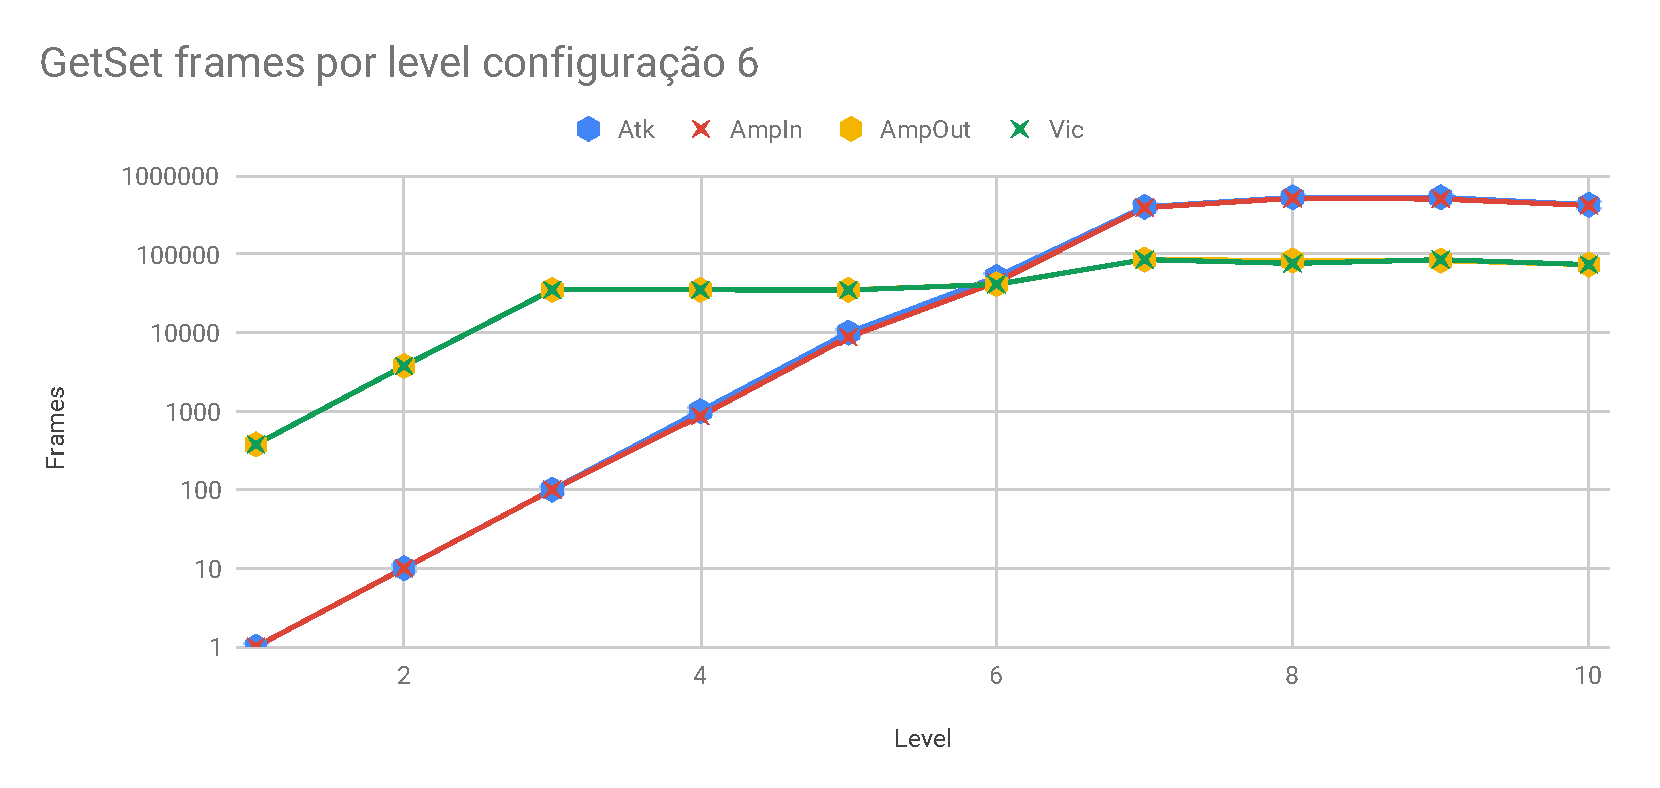
\includegraphics[scale=0.6]{img/capturas/GetSetFLC6.pdf}\
     \caption{GetSet frames por level configuração 6}
\end{figure}

\begin{table}[H]
\centering
\label{tab:bytespacsGetSet6}
\caption{Razão de bytes por pacotes para cada nível no método GetSet configuração 6}
\begin{tabular}{|c|c|c|}
\hline
Nível & Input & Output  \\ \hline
1     & 49.0  & 1440.75 \\ \hline
2     & 61.6  & 1440.78 \\ \hline
3     & 62.86 & 1440.78 \\ \hline
4     & 62.98 & 1440.78 \\ \hline
5     & 63.0  & 1440.78 \\ \hline
6     & 63.0  & 1440.81 \\ \hline
7     & 63.0  & 1440.79 \\ \hline
8     & 63.0  & 1440.8  \\ \hline
9     & 63.0  & 1440.79 \\ \hline
10    & 63.0  & 1440.79 \\ \hline
\end{tabular}
\end{table}

\subsubsection{Stats}

\begin{figure}[H]
     \centering
     \label{graf:StatsBytes6}
     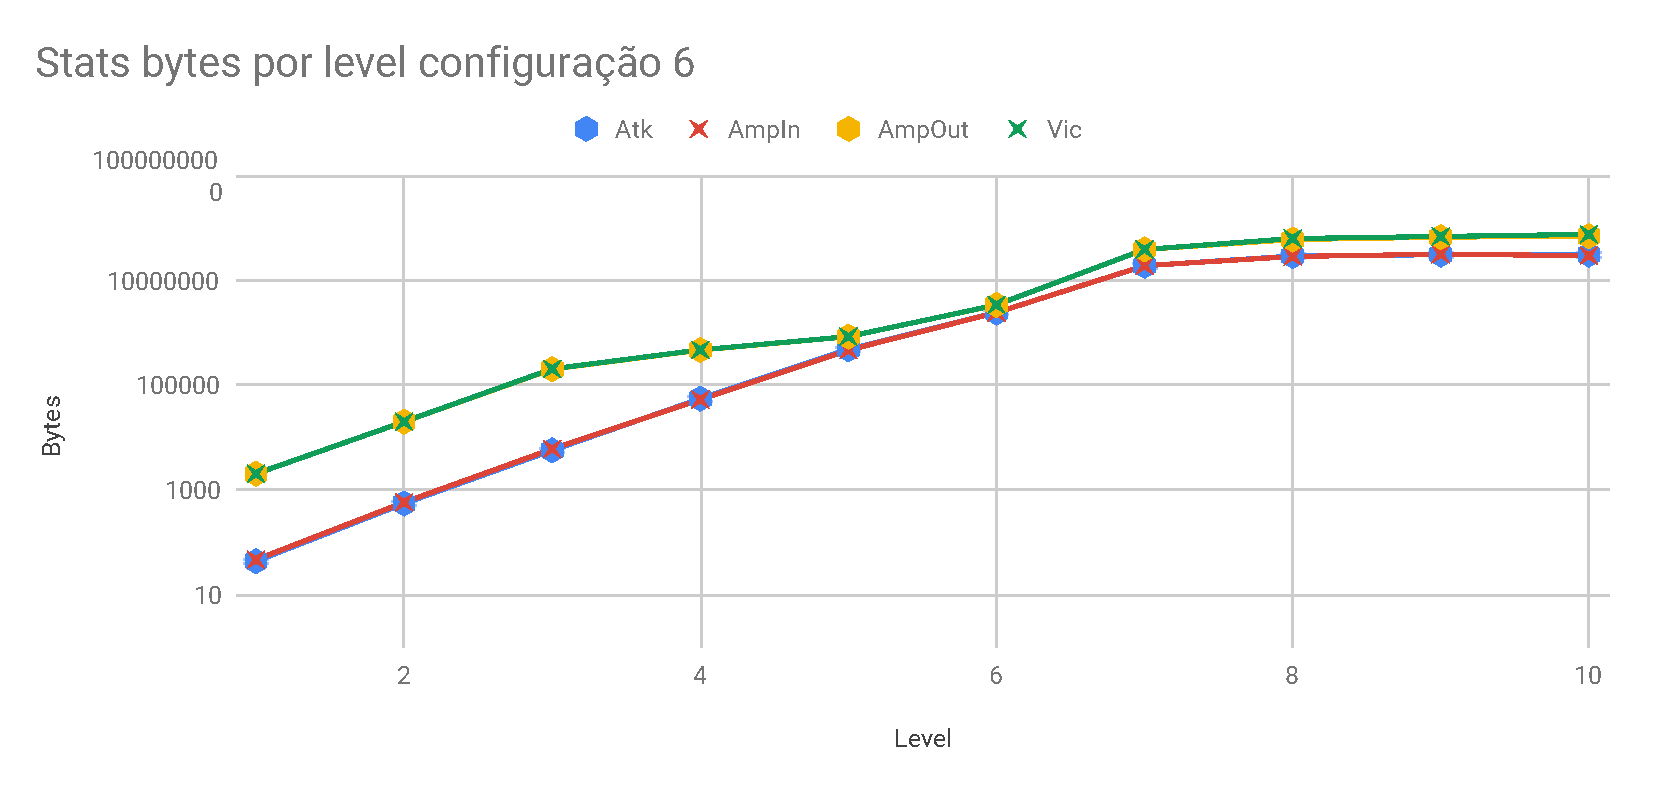
\includegraphics[scale=0.6]{img/capturas/StatsBLC6.pdf}\
     \caption{Stats bytes por level configuração 6}
\end{figure}

\begin{figure}[H]
     \centering
     \label{graf:StatsFrames6}
     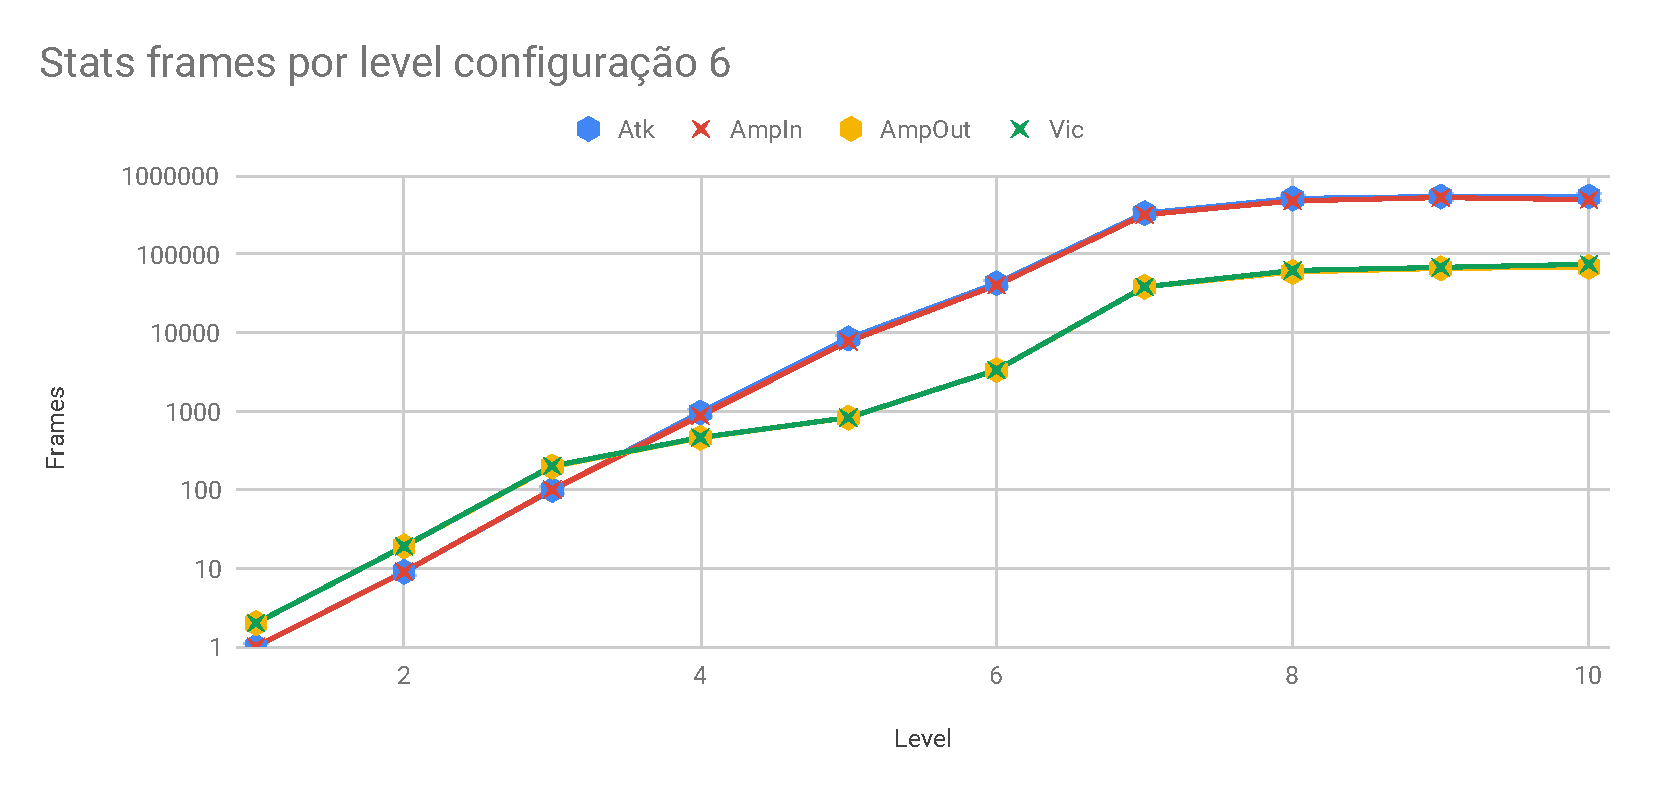
\includegraphics[scale=0.6]{img/capturas/StatsFLC6.pdf}\
     \caption{Stats frames por level configuração 6}
\end{figure}

\begin{table}[H]
\centering
\label{tab:bytespacsStats6}
\caption{Razão de bytes por pacotes para cada nível no método Stats configuração 6}
\begin{tabular}{|c|c|c|}
\hline
Nível & Input & Output  \\ \hline
1     & 46.0  & 1007.5  \\ \hline
2     & 63.78 & 1045.79 \\ \hline
3     & 59.98 & 1017.52 \\ \hline
4     & 60.0  & 1015.35 \\ \hline
5     & 60.0  & 1014.48 \\ \hline
6     & 60.0  & 1014.5  \\ \hline
7     & 60.0  & 1014.52 \\ \hline
8     & 60.0  & 1014.52 \\ \hline
9     & 60.0  & 1014.52 \\ \hline
10    & 60.0  & 1014.97 \\ \hline
\end{tabular}
\end{table}

\subsection{Amplificação}

Nessa seção iremos apresentar as tabelas de amplificação. O cálculo de amplificação apresentada nas tabelas \ref{tab:AmpBytesGetSet} e \ref{tab:AmpBytesStats} é similar a fórmula apresentada em \ref{cal:AmpFactor}. A diferença aqui é que optamos por fazer a divisão de todos os bytes recebidos pelo refletor por todos os bytes enviados pelo refletor em cada nível para facilitar a visualização de sua saturação. As tabelas \ref{tab:AmpPacGetSet} e \ref{tab:AmpPacStats} apresentam a amplificação dos pacotes de acordo com a quantidade de pacotes que chega no amplificador com a quantidade que é enviado para a vítima. 

\begin{table}[H]
\centering
\caption{Tabela de amplificação dos bytes por nível no método GetSet}
\label{tab:AmpBytesGetSet}
\begin{tabular}{|c|c|c|c|c|c|c|}
\hline
               & \multicolumn{6}{c|}{\textbf{Configuração}}                                  \\ \hline
\textbf{Nível} & \textbf{1} & \textbf{2} & \textbf{3} & \textbf{4} & \textbf{5} & \textbf{6} \\ \hline
\textbf{1}     & 11850.08   & 11084.94   & 11084.94   & 13762.94   & 11084.94   & 11084.94   \\ \hline
\textbf{2}     & 9805.64    & 8817.77    & 8817.77    & 9381.02    & 8817.77    & 8817.77    \\ \hline
\textbf{3}     & 9920.83    & 8468.22    & 8504.57    & 8933.48    & 8554.63    & 8036.17    \\ \hline
\textbf{4}     & 1044.85    & 845.13     & 862.38     & 1048.6     & 862.38     & 926.14     \\ \hline
\textbf{5}     & 108.45     & 88.09      & 87.73      & 108.63     & 92.41      & 91.39      \\ \hline
\textbf{6}     & 16.52      & 32.59      & 27.5       & 26.5       & 35.17      & 21.4       \\ \hline
\textbf{7}     & 4.71       & 10.41      & 8.93       & 7.59       & 9.89       & 5          \\ \hline
\textbf{8}     & 3.89       & 6.22       & 5.84       & 6.24       & 5.94       & 3.69       \\ \hline
\textbf{9}     & 4.07       & 6.4        & 5.93       & 6.28       & 5.7        & 3.76       \\ \hline
\textbf{10}    & 3.89       & 6.76       & 6.71       & 5.52       & 7.25       & 4.04       \\ \hline
\end{tabular}
\end{table}

\begin{figure}[H]
     \centering
     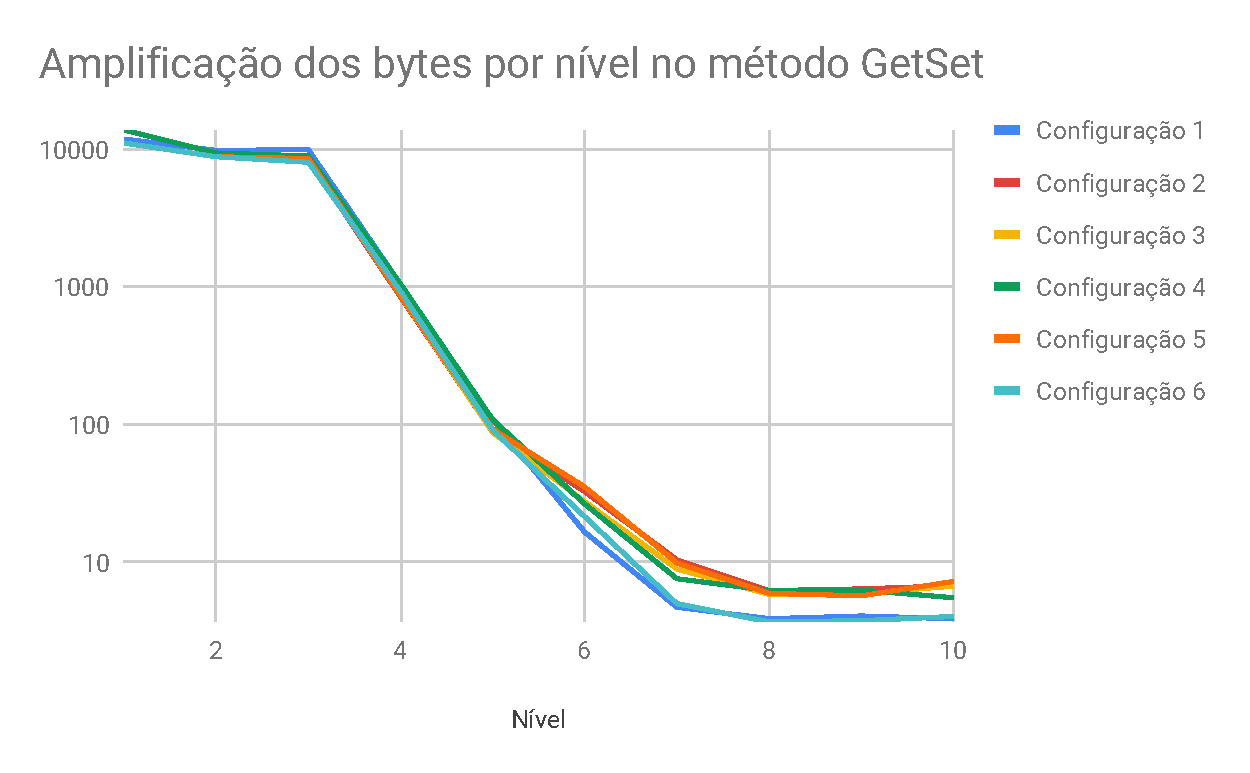
\includegraphics[scale=0.7]{img/AmppGetSet.pdf}\
     \caption{Gráfico amplificação dos bytes por nível no método GetSet}
     \label{img:GSB1}
\end{figure}

\begin{table}[H]
\centering
\caption{Amplificação dos pacotes por nível no método GetSet}
\label{tab:AmpPacGetSet}
\begin{tabular}{|c|c|c|c|c|c|c|}
\hline
               & \multicolumn{6}{c|}{\textbf{Configuração}}                                  \\ \hline
\textbf{Nível} & \textbf{1} & \textbf{2} & \textbf{3} & \textbf{4} & \textbf{5} & \textbf{6} \\ \hline
\textbf{1}     & 403        & 377        & 377        & 468        & 377        & 377        \\ \hline
\textbf{2}     & 418.11     & 377        & 377        & 418.11     & 377        & 377        \\ \hline
\textbf{3}     & 432.6      & 369.46     & 373.23     & 392.14     & 373.23     & 350.61     \\ \hline
\textbf{4}     & 45.68      & 36.95      & 37.7       & 45.84      & 37.7       & 40.49      \\ \hline
\textbf{5}     & 4.74       & 3.85       & 3.84       & 4.75       & 4.04       & 4          \\ \hline
\textbf{6}     & 0.72       & 1.43       & 1.2        & 1.16       & 1.54       & 0.94       \\ \hline
\textbf{7}     & 0.21       & 0.46       & 0.39       & 0.33       & 0.43       & 0.22       \\ \hline
\textbf{8}     & 0.17       & 0.27       & 0.26       & 0.27       & 0.26       & 0.16       \\ \hline
\textbf{9}     & 0.18       & 0.28       & 0.26       & 0.27       & 0.25       & 0.16       \\ \hline
\textbf{10}    & 0.17       & 0.3        & 0.29       & 0.24       & 0.32       & 0.18       \\ \hline
\end{tabular}
\end{table}

\begin{figure}[H]
     \centering
     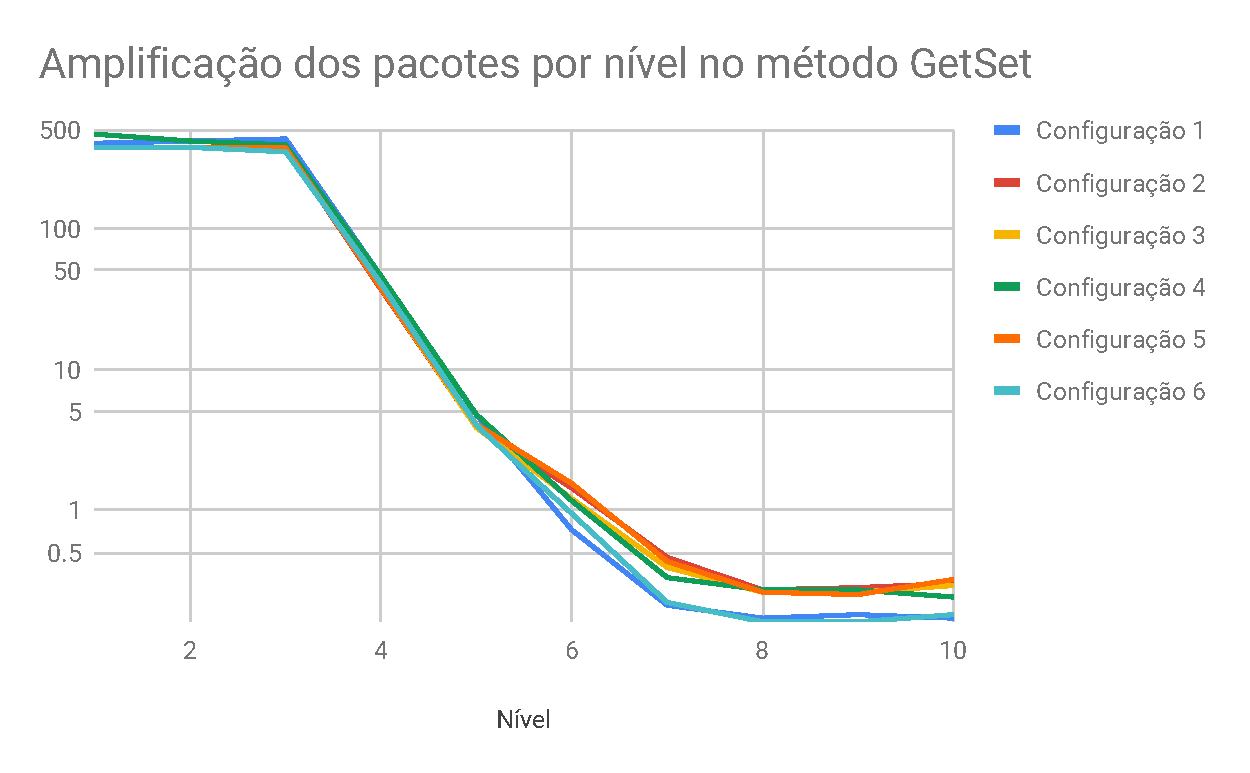
\includegraphics[scale=0.7]{img/AmppacGetSet.pdf}\
     \caption{Gráfico amplificação dos pacotes por nível no método GetSet}
\end{figure}

\begin{table}[H]
\centering
\caption{Amplificação dos bytes por nível no método Stats}
\label{tab:AmpBytesStats}
\begin{tabular}{|c|c|c|c|c|c|c|}
\hline
               & \multicolumn{6}{c|}{\textbf{Configuração}}                                  \\ \hline
\textbf{Nível} & \textbf{1} & \textbf{2} & \textbf{3} & \textbf{4} & \textbf{5} & \textbf{6} \\ \hline
\textbf{1}     & 43.26      & 43.98      & 43.78      & 41.41      & 43.93      & 43.8       \\ \hline
\textbf{2}     & 34.17      & 34.74      & 34.58      & 34.28      & 34.7       & 34.62      \\ \hline
\textbf{3}     & 33.48      & 33.35      & 33.88      & 33         & 33.65      & 33.42      \\ \hline
\textbf{4}     & 13.31      & 4.33       & 8.42       & 9.36       & 4.24       & 8.83       \\ \hline
\textbf{5}     & 2.61       & 2.37       & 2.03       & 2.61       & 2.52       & 1.81       \\ \hline
\textbf{6}     & 1.73       & 2.39       & 1.71       & 2.79       & 1.73       & 1.4        \\ \hline
\textbf{7}     & 2.46       & 2.55       & 1.22       & 2.51       & 1.28       & 2.04       \\ \hline
\textbf{8}     & 2.19       & 2.51       & 0.87       & 2.38       & 0.92       & 2.1        \\ \hline
\textbf{9}     & 2.39       & 2.52       & 0.91       & 2.52       & 0.86       & 2.12       \\ \hline
\textbf{10}    & 2.36       & 2.47       & 0.87       & 2.35       & 1          & 2.35       \\ \hline
\end{tabular}
\end{table}

\begin{figure}[H]
     \centering
     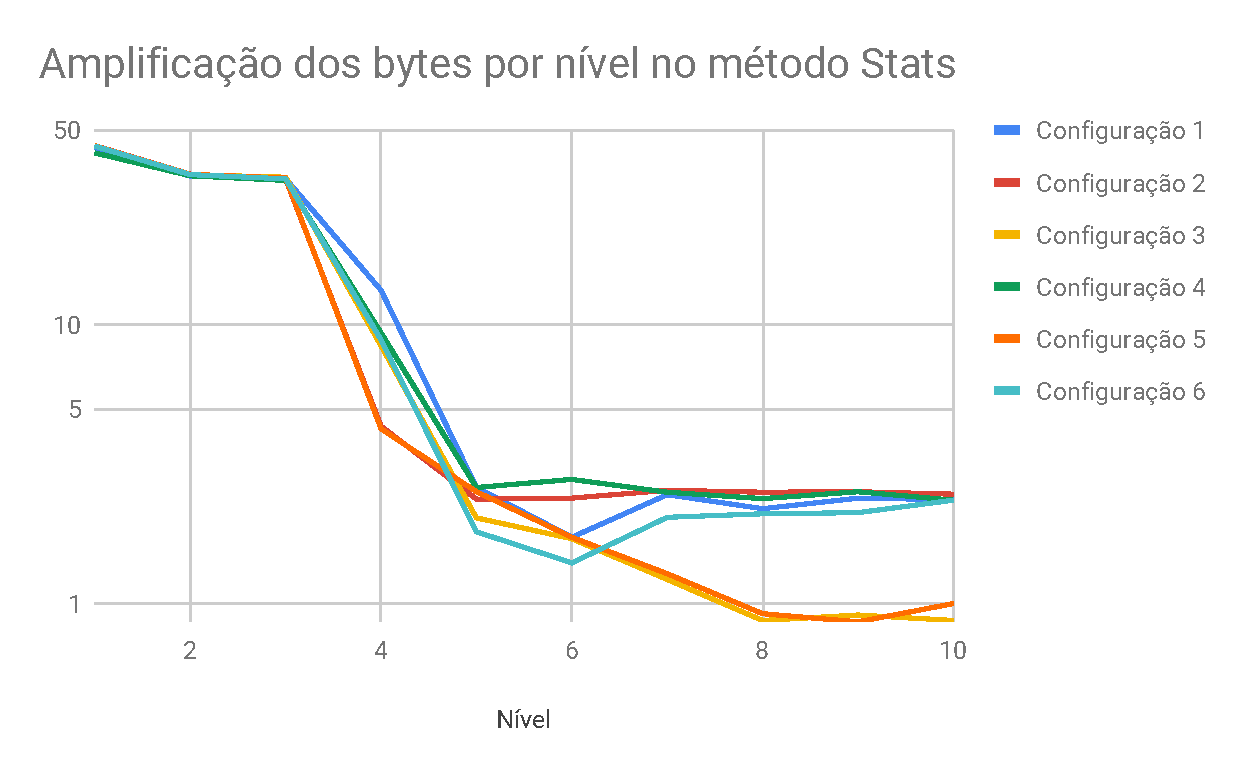
\includegraphics[scale=0.7]{img/AmpStats.pdf}\
     \caption{Gráfico amplificação dos bytes por nível no método Stats}
\end{figure}

\begin{table}[H]
\centering
\caption{Amplificação dos pacotes por nível no método Stats}
\label{tab:AmpPacStats}
\begin{tabular}{|c|c|c|c|c|c|c|}
\hline
               & \multicolumn{6}{c|}{\textbf{Configuração}}                                  \\ \hline
\textbf{Nível} & \textbf{1} & \textbf{2} & \textbf{3} & \textbf{4} & \textbf{5} & \textbf{6} \\ \hline
\textbf{1}     & 2          & 2          & 2          & 1          & 2          & 2          \\ \hline
\textbf{2}     & 2          & 2          & 2          & 1.9        & 2          & 2.11       \\ \hline
\textbf{3}     & 2          & 1.96       & 2          & 1.93       & 1.98       & 1.97       \\ \hline
\textbf{4}     & 0.8        & 0.25       & 0.5        & 0.55       & 0.25       & 0.52       \\ \hline
\textbf{5}     & 0.16       & 0.14       & 0.12       & 0.15       & 0.15       & 0.11       \\ \hline
\textbf{6}     & 0.1        & 0.14       & 0.1        & 0.16       & 0.1        & 0.08       \\ \hline
\textbf{7}     & 0.15       & 0.15       & 0.07       & 0.15       & 0.08       & 0.12       \\ \hline
\textbf{8}     & 0.13       & 0.15       & 0.05       & 0.14       & 0.05       & 0.12       \\ \hline
\textbf{9}     & 0.14       & 0.15       & 0.05       & 0.15       & 0.05       & 0.13       \\ \hline
\textbf{10}    & 0.14       & 0.15       & 0.05       & 0.14       & 0.06       & 0.14       \\ \hline
\end{tabular}
\end{table}

\begin{figure}[H]
     \centering
     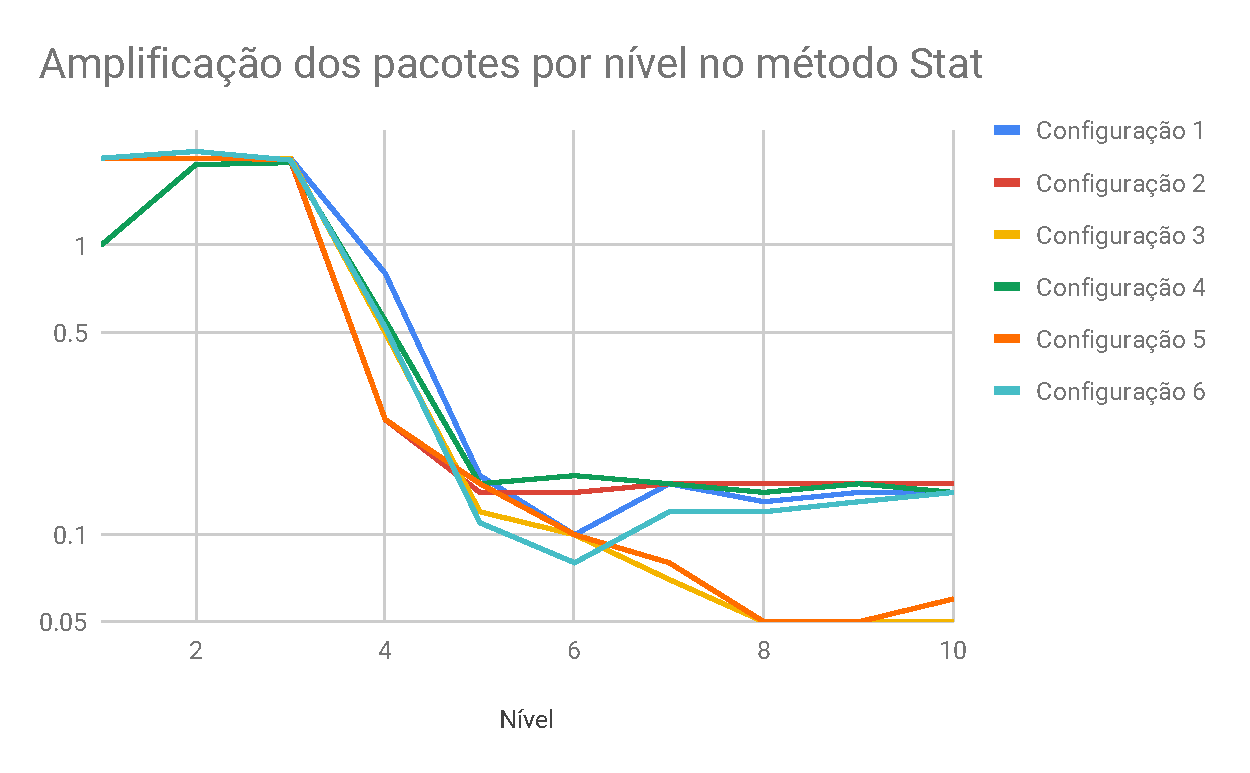
\includegraphics[scale=0.7]{img/AmppacStats.pdf}\
     \caption{Gráfico amplificação dos pacotes por nível no método Stats}
\end{figure}

\subsection{Análise da amplificação}

Ao observarmos a tabela \ref{tab:AmpBytesGetSet} vimos que nas configurações 1 e 4 foi onde tivemos as maiores amplificações no método GetSet, com a configuração 4 fornecendo a maior amplificação. Essas duas configurações possuem o refletor forte, mas são refletores diferentes, com a configuração 1 utilizando o Spitfire e a 4 o Orion. O interessante foi que essa maior amplificação não se repetiu nas configurações 2 e 6 que apresentaram uma amplificação próxima a amplificação fornecida pelo Sputnik que era a máquina mais fraca. A maior semelhança nessas configurações foi a utilização do Sputnik como atacante, mas como o atacante é responsável apenas por enviar as requisições para o atacante e utilizamos o Linderhof na execução do ataque em todas as configurações não verificamos qualquer influencia que o atacante poderia causar no refletor além de aumentar as requisições.

No método Stats a tabela \ref{tab:AmpBytesStats} mostrou que as configurações 1 e 4 geraram as menores amplificações e as configurações 2 e 6 gerando as maiores amplificações, sendo exatamente o oposto do que aconteceu no método GetSet. Isso nos mostra que o atacante realmente não influencio na amplificação no refletor.

Essa maior amplificação observada foi devido a uma maior amplificação dos pacotes que saíram do refletor, entretanto não conseguimos descobrir o motivo de tal.


\subsection{Análise de performance do atacante}

O atacante não recebe nenhum pacote, ele apenas envia para o refletor os pacotes Get ou Stats Memcached. A preparação que deve ser feita antes de começar o ataque GetSet não foi considerada na análise, já que nessa etapa do ataque não existe nenhuma amplificação, com o pacote de Set Memcached sendo muito maior que a resposta do servidor, se existir.

Ao observarmos o comportamento do atacante verificamos que ele se comportou da maneira esperada, i.e sem saturar, até o nível 7, apesar de a partir do nível 6 ele não conseguiu entregar a quantidade de pacotes desejada. Nos gráficos apresentados na seção \ref{sec:Coleta} observamos que nos níveis de 8 ao 10 a geração de pacotes começa a ficar constante, indicando a saturação no atacante. 

No log do Linderhof observamos que a máquina Sputnik conseguiu gerar os pacotes esperados até o nível 6 e as máquinas Spitfire e Orion tiveram um comportamento melhor indo até o nível 7. Esse comportamento já era esperado uma vez que o Sputnik é máquina mais fraca utilizada nos teste.

\subsection{Análise de performance do refletor}

No ataque o refletor é responsável por receber as requisições do atacante, amplifica-las e enviar para a vítima. Como utilizamos a configuração padrão do Memcached o maior valor que conseguimos armazenar no servidor é de 524288 bytes como cada requisição tendo 49 bytes já incluindo os cabeçalhos IP e UDP, já que não consideramos o cabeçalho ethernet. Isso nos da uma valor teórico para a amplificação de:

\begin{equation}
Amp = \frac{20 + 8 + 524288}{49} \approx 10700
\label{cal:Fator_Memcached2}
\end{equation}

Para o comando Stats cada pacote de requisição possui 46 bytes com a reposta tendo 2004 bytes com ambos os valores já incluindo os cabeçalhos IP e UDP. Isso nós da uma valor teórico para a amplificação de:

\begin{equation}
Amp = \frac{2004}{46} \approx 43
\label{cal:Fator_Memcached2}
\end{equation}

Ao observarmos a tabela \ref{tab:AmpBytesGetSet} verificamos que no método GetSet a amplificação no primeiro nível foi acima do esperado em todas as configurações. Isso ocorreu devido a amplificação de pacotes feita pelo servidor Memcached que observamos na tabela \ref{tab:AmpPacGetSet}. Um pacote nesse método conseguiu gerar uma alta quantidade de pacotes em retorno para a vítima, por isso observamos uma amplificação um pouco maior que a teórica. Nas configurações 1 e 4 tivemos uma maior amplificação exatamente devido a essa maior amplificação dos pacotes.

A partir do nível 2 já começamos a ter uma redução na amplificação, e no nível 4 tivemos uma acentuada redução nos bytes enviados no refletor, confirmando um início da saturação. Apesar de observarmos a volta de um crescimento na quantidade de bytes no refletor a partir do nível 7  como mostra os gráficos das configurações a amplificação continua muito baixa, não valendo a pena tal aumento, comparado com a amplificação que obtivemos nos primeiros níveis.

No método Stats tivemos um comportamento bem similar ao método GetSet. A amplificação no primeiro nível estava dentro do esperado e ocorrendo uma redução na amplificação a partir do nível 2 com a saturação ocorrendo também a partir do nível 4. Esse método também amplificou a quantidade de pacotes enviadas para o cliente de 1 para 2 pacotes na maioria das configurações, com exceção da configuração 4.mas essa amplificação não é tão relevanto quanto no método GetSet.

Como o Linderhof tenta enviar os pacotes o mais rápido possível essa queda na amplificação a partir do nível 2 em ambos os métodos pode ser devido a um descarte de pacotes pelo Memcached já que muitos dele podem com uma diferença de tempo muito curta no amplificador. 

\subsection{Análise da vítima}

A vítima apenas recebe os pacotes do refletor. Ao observarmos os gráficos que apresentam os bytes por nível vimos que os a maioria dos bytes que saem do refletor chegam na vítima.

\section{Considerações finais}

Com os testes feitos em laboratório comprovamos que o Memcached possui características para funcionar como um refletor e um amplificador que consegue alcançar altos valores de amplificação. Entretanto a amplificação não se sustentou com uma alta injeção de pacotes no servidor, sendo muito mais vantajoso para o atacante injetar até 100 pacotes por segundo.

Observamos uma queda na amplificação já na transição do nível 1 para o nível 2. Acreditamos que o motivo dessa queda foi que devido a estrutura da rede montada para os testes possuir uma baixa latência por ser local e não possuir nenhum salto entre maquinas, somado com velocidade que o Linderhof lança os pacotes fez com que alguns pacotes fossem ignorados pelo servidor Memcached por terem chegado em uma diferença de tempo muito curta.

Na versão 1.5.10 do Memcached o valor padrão para um item armazenado foi reduzida de 1Mb para 524288 bytes. Apesar disso o servidor pode estar configurado para armazenar um item com valores maiores que o padrão, sendo assim possível gerar uma amplificação ainda maior.

Como as máquinas tinham diferença de hardware optamos por fazer a rotação delas entra atacante, amplificador e vítima. Esperávamos observar uma diferença no ponto de saturação da amplificação devido a essa diferença de hardware, entretanto não foi isso que os dados coletados mostraram. Apesar de algumas configuração fornecerem uma amplificação um pouco maior os pontos de redução da amplificação e saturação foram os mesmo em todas as configurações tanto no método GetSet quanto no Stats assim como os volumes de bytes/pacotes foram bem próximos.







